\newcommand{\winw}[2]{\textsf{window}_{#1}{(#2)}}
\newcommand{\win}[1]{\textsf{window}{(#1)}}
\newcommand{\str}[1]{#1^*}
\newcommand{\prem}[1]{\textsf{prem}~#1}
\newcommand{\conc}[1]{\textsf{conc}~#1}
\newcommand{\rewHead}[3]{\textsf{rewHead}~#1~#2~#3}
\newcommand{\rewAt}[4]{\textsf{rewAt}~#1~#2~#3~#4}
\newcommand{\prefix}[2]{\textsf{prefix}~#1~#2}

\newcommand{\strentE}[1]{\rightsquigarrow_{#1}^E}
\renewcommand{\strent}[1]{\rightsquigarrow_{#1}}

\newcommand{\pFlip}[1]{\textsf{pFlip}~#1}
\newcommand{\pFlipi}[1]{\text{\textasciitilde}#1}
\newcommand{\pRev}{\textsf{pRev}}

\newcommand{\nilstr}[2]{E~#1~#2}

\newcommand{\divides}{\mid}
\newcommand{\notdivides}{\nmid}

\newcommand{\Rtape}{\ensuremath{R_{\text{tape}}}}
\newcommand{\Rtrans}{\ensuremath{R_{\text{trans}}}}
\newcommand{\Rhalt}{\ensuremath{R_{\text{halt}}}}
\newcommand{\Rsim}{\ensuremath{R_{\text{sim}}}}

\newcommand{\isSpecStateSym}[2]{\textsf{stateSym}~#1~#2}
\newcommand{\haltString}[1]{\textsf{haltingString}~#1}
\newcommand{\validCert}[1]{\textsf{validCert}~#1}
\newcommand{\validInput}[1]{\textbf{REPLACE ME}}

\newcommand{\stringForTapeHalf}{\textsf{stringForTapeHalf}}
\newcommand{\stringForConfig}{\textsf{stringForConfig}}

\newcommand{\trewwin}[6]{
  \tikzexternaldisable
  \begin{tikzpicture}
    \draw[thick] (0, 0) -- (2.25, 0);
    \draw (0.75, -0.75) -- (0.75, 0.75);
    \draw (1.5, -0.75) -- (1.5, 0.75);
    \node at (0.375, 0.375) {\ensuremath{#1}};
    \node at (0.375, -0.375) {\ensuremath{#4}};
    \node at (1.125, 0.375) {\ensuremath{#2}};
    \node at (1.125, -0.375) {\ensuremath{#5}};
    \node at (1.875, 0.375) {\ensuremath{#3}};
    \node at (1.875, -0.375) {\ensuremath{#6}};
  \end{tikzpicture}
  \tikzexternalenable
}

\newcommand*{\irewwin}[6]{\ensuremath{[#1, #2, #3]~/~[#4, #5, #6]}}
\chapter{Reducing GenNP to Parallel Rewriting}\label{chap:gennp_pr}
After defining the problem \gennp{}, 
we introduce the string-based \emph{Parallel Rewriting} (\PR{}) problem which formally captures the idea of a string tableau constrained by rewrite windows. The rest of this chapter is then devoted to formalising the tableau construction presented in Chapter~\ref{chap:informaloverview} and proving its correctness in a reduction from \gennp{} to \PR{}.

First of all, we make the informal description of \gennp{} given in the previous chapter precise.
\begin{definition}[TMGenNP]\label{def:tmgennp}
  \mnote{TMGenNP}
  \begin{align*}
    \gennp{} (\Sigma, M,  in, k', t) \defeq \exists~cert, \length{cert} \le k' \land \exists f, ({\textsf{start}}_M, \textsf{initTape}~(in \concat cert)) \rhd_M^{\le t} f, 
  \end{align*}
  where 
  \[\gennp{} : \sigtype{{\Sigma}}. (TM~\Sigma~1 \times \listsof{\Sigma} \times \nat \times \nat) \rightarrow \Prop \]
  and 
  \begin{align*}
    \mnotec{\textsf{initTape}}~[] \defeq \textsf{niltape} \\
    \textsf{initTape}~(x::xs) \defeq \textsf{leftof}~x~xs,
  \end{align*}
  that is, the head is initially positioned left of the input.
\end{definition}

Syntactically, it is important that the numbers $t$ and $k'$ are given in a unary encoding instead of a binary encoding: with a binary encoding, a verifier for \gennp{} could not even take time linear in the number of steps. 

\section{Parallel Rewriting}\label{sec:pr}
Parallel Rewriting works over a finite alphabet $\Sigma$. Given an initial string $x_0$, a set of rewrite windows $R$, a number of steps $t$, and a final constraint $\Rfinal$, we are tasked with determining whether there exists a sequence of valid rewrites $x_0 \strent{} \ldots \strent{} x_t$ such that $x_t$ satisfies a substring constraint $\Rfinal$, written $x_t \models \Rfinal$.

\begin{definition}[Parallel Rewriting instances]\label{def:pr}
  \mnote{\PR{} instances}
  $p = (\Sigma, o, w, x_0, R, \Rfinal, t)$ is a Parallel Rewriting instance, where 
  \begin{itemize}
    \item $\Sigma : \textsf{finType}$ is the finite alphabet,
    \item $o : \nat$ with $o > 0$ is the rewriting offset,
    \item $\omega : \nat$ with $\omega > 0$ and $o \divides \omega$ is the width of rewriting windows,
    \item $x_0 : \str{\Sigma}$ with $\length{x_0} \ge \omega$ and $o \divides \length{x_0}$ is the initial string, 
    \item $R : \listsof{\winw{\omega}{\Sigma}}$ is the set of rewrite windows,
    \item $\Rfinal : \listsof{\str{\Sigma}}$ is a set of final substrings,
    \item $t : \nat$ is the number of rewrite steps.
  \end{itemize}
  Here, $\winw{\omega}{\Sigma} := {\Sigma}^\omega \times {\Sigma}^\omega$\mnote{$\winw{\omega}{\Sigma}$} denotes the type of windows of width $w$ over $\Sigma$.
\end{definition}
If it is clear from the context, we write $\win{\Sigma}$ instead of $\winw{\omega}{\Sigma}$, omitting the width.
Instead of directly using the projections $\pi_1$ and $\pi_2$ on a window $w$, we usually write $\prem{w}$ and $\conc{w}$\mnote{$\prem, \conc$}. 

Pictorially, $o$ symbols are always grouped together to form one abstract symbol, explaining the divisibility constraints. Throughout this chapter, we always work with an offset of 1 and the more general case will only become relevant in Chapter~\ref{chap:pr_bpr}.

Let us fix the structural parameters $\Sigma$, $o$ and $\omega$ satisfying the conditions stated in the definition for the rest of this section.

\subsection{Validity}
We start by defining what it means for a string $a$ to validly rewrite to another string $b$, denoted as $a \strent{} b$.
\begin{definition}[Matching Windows]\label{def:rewHead}
  \mnote{\textsf{rewHead}}
  \begin{gather*}
    \rewHead{w}{a}{b} \defeq \prefix{(\prem{w})}{a} \land \prefix{(\conc{w})}{b} \\
    \prefix{s}{t} \defeq \exists b, t = s \concat{} b,
  \end{gather*}
  \mnote{\textsf{prefix}}
  that is, a window $w$ justifies a rewrite at the head of two strings $a$ and $b$ if it matches the heads of $a$ and $b$.

  A windows $w$ justifies a rewrite at position $i$ of strings $a, b$ if it matches the head of the strings starting from position $i$:
  $\rewAt{w}{i}{a}{b} \defeq \rewHead{w}{a[i..]}{b[i..]}$
  \mnote{\textsf{rewAt}}
\end{definition}
\todo{maybe mention the facts (tail invariance, ...) which are routinely used?}

Intuitively, a rewrite $a \strent{} b$ is possible if we can find a rewrite window jusifying a local rewrite for every possible offset. ``Possible offsets'' are those in the range $[0, \length{a} - \omega]$, as the windows have a width of $\omega$. Additionally, we only need rewrites at multiples of the offset, again supporting the view that $o$ symbols together form a unit.

\begin{definition}[Validity (Explicit Characterisation)]
  Given a set of rewrite windows $R$, the validity of a rewrite of $a : \str{\Sigma}$ to $b : \str{\Sigma}$, written \mnotec{$a \strentE{R} b$}, is defined by:
  \begin{align*}
    a \strentE{R} b \defeq \quad& \length{a} = \length{b} \\
    \land \quad & (\exists k, \length{a} = k \cdot o) \\
    \land \quad & \forall 0 \le i = j \cdot o \le \length{a} - \omega, \exists w, w \in R \land \rewAt{w}{i}{a}{b} 
  \end{align*}
\end{definition}

Note that the dependency on $o$ and $\omega$ is not made explicit in the notation, instead they need to be inferred from the context. If the set of rewrite windows $R$ is clear, we may also drop that.

While this definition is fairly intuitive, it does not support easy inductive reasoning. Therefore, we use an equivalent inductive definition.

\begin{definition}[Validity] 
  Given a set of rewrite windows $R$, the validity of a rewrite of $a : \str{\Sigma}$ to $b : \str{\Sigma}$, written \mnotec{$a \strent{R} b$}, is defined inductively:  
  \begin{gather*}
    \infer{\nil \strent{R} \nil}{} \\
    \infer{u\concat{} a \strent{R} v \concat{} b}{a \strent{R} b \quad \length{a} < \omega - o \quad \length{u} = o \quad \length{v} = o} \\
    \infer{u \concat{} a \strent{R} v \concat{} b}{a \strent{R} b \quad \length{u} = o \quad \length{v} = o \quad w \in R \quad \rewHead{w}{(u\concat{}a)}{(v \concat{} b)}}.
  \end{gather*}
\end{definition}

This version prepends a chunk of $o$ symbols in each step. The first two cases deal with proving validity of rewrites in strings of length $< \omega$. The third case is the interesting one and is defined in the intuitive way.

\begin{remark}
  It might seem peculiar that we do not require the strings to have a minimum length of $\omega$: strings of length $< \omega$ can be rewritten vacuously to any other string as they are covered by no window. 
  This enables us to only mention $\textsf{rewHead}$ in the successor case of the inductive definition; otherwise, we would also need it in the base case. The main proofs of this chapter are simplified considerably by this choice, albeit at the cost of having nonsensical base cases.
\end{remark}

\begin{proposition}[Vacuous Rewriting]\label{lem:vacuous}
  Let $a, b : \str{\Sigma}$ with $\length{a} = \length{b} = k \cdot o < \omega$. Then $a \strent{} b$. 
\end{proposition}
\begin{proof}
  By induction on $k$.
\end{proof}

\begin{proposition}[Length Invariance]
  Let $a, b : \str{\Sigma}$ with $a \strent{} b$. Then $\length{a} = \length{b}$. 
\end{proposition}

\begin{lemma}[Agreement of $\strentE{}$ and $\strent{}$]\label{lem:agree_valid}
  For any set of rewrite windows $R$, it holds that 
  \[a \strentE{R} b \leftrightarrow a \strent{R} b. \]
\end{lemma}
\begin{proof}
  \begin{description}
    \item[$\rightarrow$:]
      By definition, we have $k$ with $\length{a} = k \cdot o$. The proof is by induction on $k$ with $a$ and $b$ quantified.
    \item[$\leftarrow$:]
      By induction on $a \strentE{R} b$. 
  \end{description}
\end{proof}

\subsection{The Parallel Rewriting Problem}
Parallel Rewriting generates a sequence of strings according to $\strent{R}$ for a set of rewrite windows $R$. The last string should contain one element of a set of strings $\Rfinal$ as a substring.
\begin{definition}[Substring constraint]
  Given a set of strings $\Rfinal : \listsof{\str{\Sigma}}$, string $s$ satisfies $\Rfinal$, written \mnotec{$s \models \Rfinal$}, if:
  \[\exists \mathit{subs}~k, \mathit{subs} \in \Rfinal \land k \cdot o \le \length{s} \land \prefix{\mathit{subs}}{s[k \cdot o..]} \]
\end{definition}
The definition requires a string to be a substring at a position which is a multiple of the offset $o$.

\begin{definition}[Parallel Rewriting]
  \mnote{\PR{}}
  \[\PR{}~(\Sigma, o, \omega, x_0, R, \Rfinal, t) \defeq \exists x_t, x_0 \strent{R}^t x_t \land x_t \models \Rfinal, \]
  where we implicitly require the instance to satisfy the syntactic constraints of Definition~\ref{def:pr}. 
\end{definition}

One can interpret \PR{} to be a problem between Turing machines and circuits: of course, the definition over a finite alphabet still closely resembles Turing machines. However, in contrast to Turing machines, Parallel Rewriting can completely rewrite the string in a single step, although the power of this is limited as it operates on strings of a fixed size. 
Circuits, on the other hand, are similar in the sense that they also work in parallel. The fact that adjacent rewrite positions overlap and can thus enforce a global constraint in a single rewrite step is unlike circuits, though. 

\subsection{3-\PR{}}\label{sec:3pr}
For the rest of this chapter, we fix the width $\omega$ to $3$ and the offset $o$ to $1$, which are the parameters needed for the Turing machine encoding. We call this variant 3-\PR{}. 
The inductive definition of validity can be simplified a bit:
\mnote{$a \strent{R} b$}
\begin{align*}
  \infer{\nil \strent{R} \nil}{} \quad
  \infer{x::a \strent{R} y ::b}{a \strent{R} b \quad \length{a} < 2} \quad
  \infer{x::a \strent{R} y :: b}{a \strent{R} b \quad w \in R \quad \rewHead{w}{(x::a)}{(y::b)}}
\end{align*}

We use the notation introduced in the previous chapter to denote the window $((x_1, x_2, x_3), (x_4, x_5, x_6))$: 
\begin{center}
  \trewwin{x_1}{x_2}{x_3}{x_4}{x_5}{x_6}
\end{center}
Sometimes, we also use $\irewwin{x_1}{x_2}{x_3}{x_4}{x_5}{x_6}$ if we need to write down a window in-line.

\section{Encoding Tapes and Configurations}
We start with the construction of the Turing machine simulation. Our goal is to devise and verify a 3-\PR{} instance simulating a given Turing machine. 
For the rest of the chapter, let us fix a \gennp{} instance consisting of a finite tape alphabet $\Sigma$, a single-tape Turing machine $M = (Q, \delta, \textsf{start}, \textsf{halt})$ over $\Sigma$, an input $in$, a number $t$ of steps, and a maximum size $k'$ of the certificate. 

\begin{definition}
  $\validCert~c \defeq \length{c} \le k' \mnote{$\validCert$}$
\end{definition}

Formalising the intuitions from Chapter~\ref{chap:informaloverview}, we define the alphabet $\Gamma$ of the Parallel Rewriting instance for the deterministic simulation\footnote{This does not include the part for generating the initial configuration.}.

\newcommand{\stateSigma}{\Sigma_{\mathit{state}}}
\newcommand{\delimSigma}{\Sigma_{\mathit{delim}}}
\newcommand{\tapeSigma}{\Sigma_{\mathit{tape}}}
\newcommand{\States}{\textsf{States}}

\begin{align*}
  \polarity : \Type &\defeq + \bnfmid - \bnfmid \circ \\
  \textsf{delim} : \Type &\defeq \# \\
  \stateSigma &\defeq \opt{\Sigma} \mnote{$\stateSigma$}\\
  \States &\defeq Q \times \stateSigma \mnote{$\States$}\\
  \tapeSigma &\defeq \polarity \times \stateSigma \mnote{$\tapeSigma$}\\
  \delimSigma &\defeq \textsf{delim} + \tapeSigma \mnote{$\delimSigma$}\\
  \Gamma &\defeq \States + \delimSigma
  \mnote{$\Gamma$}
\end{align*}

We need the subalphabets at various points. When we write down elements of $\Gamma$, we leave the injections into the sum types and option types implicit. Sometimes, we also implicitly lift functions from a smaller alphabet to a larger one.
We use the metavariables $\sigma : \Sigma$, $m : \tapeSigma$, $p : \polarity$, $\gamma : \Gamma$, $u : \str{\Sigma}$, and $h : \str{\Gamma}$. 
\mnote{$\polneg{m}, \polpos{m}, \polneut{m}$}
Given $m$, we write $\polpos{m}$ for $(+, m)$, $\polneg{m}$ for $(-, m)$, and $\polneut{m}$ for $(\circ, m)$. For an unknown polarity $p$, we use \mnotec{$m^p$}.

\begin{definition}[Polarity Reversion]
  \begin{align*}
    \pFlip{p} &\defeq \match p \withl \circ~\Rightarrow \circ \withm +~\Rightarrow - \withm -~\Rightarrow +\withr \\
    \pRev~(h : \str{\Gamma}) : \str{\Gamma} &\defeq \rev{\withl\pFlip{x} \bnfmid x \in h\withr}
    \mnote{\pRev}
  \end{align*}
  Notationally, we write \mnotec{$\pFlipi{p}$} for $\pFlip{p}$. 
\end{definition}
$\pRev$ reverses a string and flips the polarities the symbols are annotated with.
Note that we are already using an implicit lifting of $\pFlip{}$ from \polarity{} to $\Gamma$ in the definition of $\pRev$. 

\begin{fact}[Involutions]\label{fact:prev_involution}
  $\pFlip{}$ and $\pRev{}$ are involutions, that is, $\pFlip{(\pFlip{p})} = p$ and $\pRev{(\pRev~h)} = h$. 
\end{fact}

Figure~\ref{fig:configlayout} shows the layout of a configuration string again. We refer to the center symbol as the \emph{state symbol} and to the substrings left and right of it as the \emph{left tape half} and the \emph{right tape half}.
In dependence of $t$, $k'$, and $in$, we define the following numbers:
\begin{align*}
  k &\defeq \length{in} + k' \\
  z &\defeq t + k \mnote{z}\\
  \forall n, \hat{n} &\defeq n + 2 \mnote{$\hat{n}$}\\
  l &\defeq 2 \cdot (\hat{z} + 1) + 1 \mnote{l}
\end{align*}
The real maximum input size after accounting for the fixed input $in$ and the nondeterministic certificate is $k$.
$z$ is the amount of space available for the Turing machine and thus $z$ units of space need to be available to the left and to the right in the configuration string as the tape can be shifted to be completely on one side of the state symbol.
For technical reasons, we want three symbols to be available to either side of the state symbol even if $t = k = 0$. One of those symbols is the delimiter $\#$, the other two are additional blanks which will never be used by the Turing machine. Thus $\hat{z}$ is the number of symbols on each side excluding the delimiter. 
Finally, $l$ is the length of the whole configuration string including the center state symbol.

\begin{figure}
  \begin{center}
    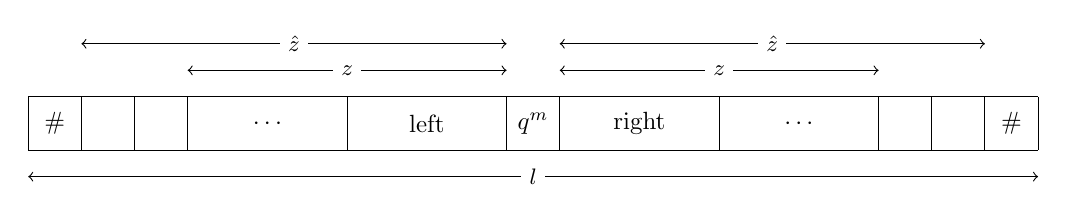
\begin{tikzpicture}[scale=0.9, every node/.style={scale=0.9}]
      \draw (-1.5, 0) -- (12.75, 0);
      \draw (-1.5, 0) -- (-1.5, 0.75);
      \draw (-1.5, 0.75) -- (12.75, 0.75);
      \draw (12.75, 0.75) -- (12.75, 0);

      \draw (0.75, 0) -- (0.75, 0.75);
      \draw (10.5, 0) -- (10.5, 0.75);
      \draw (0, 0) -- (0, 0.75);
      \draw (11.25, 0) -- (11.25, 0.75);
      \draw (-0.75, 0) -- (-0.75, 0.75);
      \draw (12, 0) -- (12, 0.75);

      \draw (6, 0) -- (6, 0.75);
      \draw (5.25, 0) -- (5.25, 0.75);

      \draw (3, 0) -- (3, 0.75);
      \draw (8.25, 0) -- (8.25, 0.75);

      \node at (-1.125, 0.375) {\#};
      \node at (-0.375, 0.375) {\blank};
      \node at (0.375, 0.375) {\blank};
      \node at (5.625, 0.375) {$q^m$};
      \node at (12.375, 0.375) {\#};
      \node at (11.625, 0.375) {\blank};
      \node at (10.875, 0.375) {\blank};

      \node at (1.125, 0.375) {\blank};
      \node at (1.875, 0.375) {$\cdots$};
      \node at (2.625, 0.375) {\blank};

      \node at (8.625, 0.375) {\blank};
      \node at (9.375, 0.375) {$\cdots$};
      \node at (10.125, 0.375) {\blank};

      \node at (4.125, 0.375) {left};
      \node at (7.125, 0.375) {right};
      
      \path[<->] (-0.75, 1.5) edge node[fill=white, anchor=center, pos= 0.5] {\small $\hat{z}$} (5.25, 1.5);
      \path[<->] (0.75, 1.125) edge node[fill=white, anchor=center, pos=0.5] {\small $z$} (5.25, 1.125);
      \path[<->] (6, 1.5) edge node[fill=white, anchor=center, pos= 0.5] {\small $\hat{z}$} (12, 1.5);
      \path[<->] (6, 1.125) edge node[fill=white, anchor=center, pos=0.5] {\small $z$} (10.5, 1.125);
      \path[<->] (-1.5, -0.375) edge node[fill=white,anchor=center, pos=0.5] {\small $l$} (12.75, -0.375);


    \end{tikzpicture}
  \end{center}
  \caption{Layout of a configuration string.}\label{fig:configlayout}
\end{figure}


In order to make reasoning about configuration strings possible, we define representation relations for tape halves and configurations.

\begin{definition}[Tape Representation]
  The string $E$ represents the empty tape: 
  \mnote{$\nilstr{p}{n}$}
  \begin{align*}
    \nilstr{p}{0} &\defeq [\#] \\
    \nilstr{p}{(\natS{n})} &\defeq (p, \blank) :: \nilstr{p}{n}
  \end{align*}
  Tape representation is defined as:
  \mnote{$u \reprtt{n}{p} h$}
  \begin{align*}
    u \reprtt{n}{p} h &\defeq \length{u} \le n \land h = \withl(p, x) \withm x \in u\withr \concat \nilstr{p}{(\hat{n} - \length{u})}\\
  u \reprt{p} h &\defeq u \reprtt{z}{p}, \mnote{$ u \reprt{p} h$}
  \end{align*}
\end{definition}
$u \reprtt{n}{p} h$ means that $h$ contains the elements of $u$ annotated with polarity $p$ where a total of $n$ symbols are available for the simulation to use.
For the correctness statements, we use $u \reprt{p} h$, but usually generalise to $u \reprtt{n}{p} h$ for some $n$ in inductive proofs. 

\begin{proposition}\label{prop:tapefacts}\leavevmode
  \begin{itemize}
    \item $\withl \pFlip{\gamma} \withm \gamma \in \nilstr{p}{n} \withr = \nilstr{(\pFlip~p)}{n}$
    \item $u \reprtt{n}{p} h \rightarrow \length{h} = \natS{\hat{n}}$
    \item $u \reprtt{n}{p} h \rightarrow u \reprtt{n}{\pFlip{p}} \withl \pFlip{\gamma} \withm \gamma \in h \withr$
  \end{itemize}
\end{proposition}
\todo{maybe unique representation of the empty tape}

\begin{definition}[Configuration Representation]
  \begin{align*}
    \mnote{$ (q, tp) \reprc{} (l, e, r)$}
    (q, tp) \reprc{} (l, e, r) &\defeq \exists p, e = (q, \tmcurrent{tp}) \land \tmleft{tp} \reprt{p} l \land \tmright{tp} \reprt{p} r \\
    c \reprc{} s &\defeq \exists l~ e~ r, s = \rev~{l} \concat{} [e] \concat{} r \land (q, tp) \reprc{} (l, e, r) \mnote{$ (q, tp) \reprc{} s$}
  \end{align*}
\end{definition}
A configuration $c = (q, tp)$ is represented by a string containing the state symbol at the center with strings representing the left and right tape halves left and right of it. Note that the left tape half is reversed: while the Turing machine tapes have the symbol closest to the machine head at the head of the list, we need the symbol closest to the head to be next to the string's center. This will pose some difficulties later on.


\mnote{$\stringForTapeHalf$}
Both $\reprt{}$ and $\reprc{}$ are computational in the sense that, given a tape half or a configuration, respectively, we can compute a string representing this tape half or configuration. 
Let $\stringForTapeHalf : \str{\Sigma} \rightarrow \str{\Gamma}$ and $\stringForConfig : Q \rightarrow \textsf{tape}~(\Sigma) \rightarrow \str{\Gamma}$ be such functions.
\mnote{$\stringForConfig$}

\section{Modifying Tapes}\label{sec:taperules}
In this section, we introduce the rewrite rules for shifting tape halves and prove the main results for manipulating the representation of a tape half.

\subsection{Tape Rules}
Recall that we need rules for shifting the tape to the left, to the right, or leaving its position unchanged.
The rules are annotated with the tape halves they can be used on. These annotations have no formal meaning but help with the intuition.

\paragraph{Right Shifts}
\begin{center}
\begin{tabular}{cc}
\trewwin{\sigma_1}{\sigma_2}{\sigma_3}{\polpos{\sigma_4}}{\polpos{\sigma_1}}{\polpos{\sigma_2}} 
  \quad \trewwin{\blank}{\blank}{\blank}{\polpos{\blank}}{\polpos{\blank}}{\polpos{\blank}}
  & (both halves) \\
\trewwin{\blank}{\blank}{\blank}{\polpos{\sigma_1}}{\polpos{\blank}}{\polpos{\blank}} 
  \quad \trewwin{\sigma_1}{\blank}{\blank}{\polpos{\sigma_2}}{\polpos{\sigma_1}} {\polpos{\blank}}
\quad \trewwin{\sigma_1}{\sigma_2}{\blank}{\polpos{\sigma_3}}{\polpos{\sigma_1}}{ \polpos{\sigma_2}}
  & (right half) \\
\trewwin{\blank}{\blank}{\sigma_1}{\polpos{\blank}}{\polpos{\blank}}{\polpos{\blank}}
  \quad \trewwin{\blank}{\sigma_1}{\sigma_2} {\polpos{\blank}}{\polpos{\blank}}{ \polpos{\sigma_1}} 
\quad \trewwin{\sigma_1}{\sigma_2}{\sigma_3}{\polpos{\blank}}{\polpos{\sigma_1}}{ \polpos{\sigma_2}}
  & (left half)
\end{tabular}
\end{center}
\todo{fix formatting}

The rules implicitly encode the invariant that all symbols used by the Turing machine are placed contiguously with no blanks inbetween. For instance, we do not need the following two rules:
\begin{center}
  \trewwin{\sigma_1}{\blank}{\sigma_2}{\polpos{\blank}}{\polpos{\sigma_1}}{\polpos{\blank}}
  \quad
  \trewwin{\sigma_1}{\blank}{\blank}{\polpos{\blank}}{\polpos{\sigma_1}}{\polpos{\blank}}
\end{center}
In the first case, the premise prevents the rule from ever being applicable. In the second case, the overlap of the rewrite windows and the state symbol which stands between both tape halves makes it impossible to have the substring $\blank \polpos{\sigma_1} \blank$. 
We call such instantiations of a rewrite rule \emph{spurious}.

Knowing this, we write down the above rules in a more succinct way as 
\begin{center}
  \trewwin{m_1}{m_2}{m_3}{\polpos{m_4}}{\polpos{m_1}}{\polpos{m_2}}
\end{center}
While we would be fine having the spurious rewrite windows, they do make additional reasoning necessary in some cases. Therefore, we just regard this as a notation for the expanded form above, instead of actually having the spurious instantitions. One can easily derive the rules which are actually relevant.

\paragraph{Left Shifts}
We only write down the abbreviated form:
\begin{center}
  \trewwin{m_1}{m_2}{m_3}{\polneg{m_2}}{\polneg{m_3}}{\polneg{m_4}}
\end{center}
Note that this rule exactly mirrors the rule for shifting the tape to the right.

\paragraph{Identity Rules}
\begin{center}
  \trewwin{m_1}{m_2}{m_3}{\polneut{m_1}}{\polneut{m_2}}{\polneut{m_3}}\\
  \trewwin{\#}{\blank}{\blank}{\#}{\blank}{\blank} 
  \quad \trewwin{\blank}{\blank}{\#}{\blank}{\blank}{\#}
\end{center}
We need no windows which contain both the delimiter $\#$ and an element of $\Sigma$ as the Turing machine (by construction of $z$) cannot use the two blanks adjacent to the delimiters within the number of steps it is given.

The collection of all windows generated by these rules is referred to as \mnotec{$\Rtape$}.

\begin{remark}
  It now becomes clear why we need the delimiter $\#$. Without it, symbols could just be introduced at the edge of the string. For instance, the rule 
  \begin{center}
    \tikzset{baseline={([yshift=-22pt]current bounding box.north)}}
    \trewwin{\blank}{\blank}{\blank}{\polpos{\sigma_1}}{\polpos{\blank}}{\polpos{\blank}},
  \end{center}
  which is intended for use on the right tape half, could then also be used at the leftmost position of the left tape half as no rewrite window is overlapping from the left.
\end{remark}

\begin{lemma}[Symmetry of \Rtape]\label{lem:symm_rtape}
  \[\irewwin{\gamma_1}{\gamma_2}{\gamma_3}{\gamma_4}{\gamma_5}{\gamma_6} \in \Rtape \leftrightarrow \irewwin{\pFlipi{\gamma_3}}{\pFlipi{\gamma_2}}{\pFlipi{\gamma_1}}{\pFlipi{\gamma_6}}{\pFlipi{\gamma_5}}{\pFlipi{\gamma_4}} \in \Rtape \]
\end{lemma}
\begin{proof}
  We first prove one direction and then use that $\pFlip$ is involutive (Fact~\ref{fact:prev_involution}).
  By inversion on the rule used to generate the window. The interesting case is the one for shifting the tape to the left or to the right, which follows by the fact that the rules for shifting to the left and shifting to the right are exactly symmetric. 
\end{proof}

The following lemma will be extremely helpful in the sequel.
If we want to prove a statement for the left and the right tape half, it allows us to just prove the statement for the right tape half and then get the symmetric result for the left tape half for free. This is useful in particular because we cannot do direct inductions over the reversed left tape half. 

%lemma 15 from memo
\begin{lemma}[Symmetry of Tape Rewrites]\label{lem:symm_tape_rew}\leavevmode
  \begin{enumerate}
    \item $h \strent{\Rtape} h' \rightarrow \pRev~h \strent{\Rtape} \pRev~h'$ 
    \item $\pRev~h \strent{\Rtape} \pRev~h' \rightarrow h \strent{\Rtape} h'$
    \item $h \strent{\Rtape} h' \rightarrow \withl \pFlip{x} \withm x \in h \withr \strent{\Rtape} h'$
  \end{enumerate}
\end{lemma}
\begin{proof}
  \begin{enumerate}
    \item By induction on $h \strent{\Rtape} h'$. The first two cases are trivial. 
      In the successor case, there is the problem that the new symbols are appended at the end of the strings, while the inductive definition of $\strent{}$ only allows to prepend new symbols. We switch to the explicit characterisation by Lemma~\ref{lem:agree_valid} and do a case analysis on the position for which we need to provide a rewrite window. For all but the last position, we can apply the inductive hypothesis, while we use the polarity-reversed new rewrite window, which exists by Lemma~\ref{lem:symm_rtape}, for the last position.
    \item Apply 1.\ and use that $\pRev$ is an involution.
    \item By induction on $h \strent{\Rtape} h'$ and inversion on the used rewrite rule.
  \end{enumerate}
\end{proof}


\subsection{Manipulation of Blank Tape Representations}

We prove several lemmas which are similar in flavour and will later be the base cases of more general results. They state that, starting from a blank tape half, we can leave the tape half unchanged, add a symbol of $\Sigma$, or remove a symbol that prefixes it. Moreover, if a blank tape half rewrites to a string of which the first symbol is known, the rest of the string is also uniquely determined. This is just an instance of the more general observation that the rewrite rules introduced up to now only allow for deterministic rewrites.
These results are each proven for the right tape half and then derived for the left tape half by Lemma~\ref{lem:symm_tape_rew}. 

\begin{remark}
  It now becomes clear why we require at least three symbols on each side of the state symbol: this way, we can prove results about each of the tape halves individually without running into the problem of vacuous rewrites~(Lemma~\ref{lem:vacuous}). 
\end{remark}

%lemma 16
\begin{lemma}[Empty Tape Half: Blank Rewriting]\label{lem:nilstr_blank}\leavevmode
  \begin{enumerate}
    \item $\nilstr{p}{\hat{n}} \strent{\Rtape} \nilstr{p'}{\hat{n}}$ and $\nilstr{p}{\hat{n}} \strent{\Rtape} (p', \blank) :: s \rightarrow s = \nilstr{p'}{(\natS{n})}$
    \item $\rev~{(\nilstr{p}{\hat{n}})} \strent{\Rtape} \rev~{(\nilstr{p}{\hat{n}})}$ and $\rev~{(\nilstr{p}{\hat{n}})} \strent{\Rtape} \rev~{((p', \blank) :: s)} \rightarrow s = \nilstr{p'}{(\natS{n})}$
  \end{enumerate}
\end{lemma}
\begin{proof}
  \begin{enumerate}
    \item The first statement follows by induction on $n$. For the second one, we unfold $\hat{n} = \natS{(\natS{n})}$ and generalise $\natS{n}$ to arbitrary $n \ge 1$. The statement then follows by induction on $n$: the base case is contradictory. In the successor case, we do another case analysis on $n$. If $n =0$, the statement follows by inversion on the used rewrite rule. 
      Otherwise, $n = \natS{n'}$. We have $\nilstr{p}{(3+n')} \strent{} (p', \blank) :: s$ and show $s = \nilstr{p'}{(2 + n)}$. By inversion on the rewrite rule used at the head, we get four cases and in each one, $s = (p', \blank) :: s'$ and $\nilstr{p}{(2+n)} \strent{} (p', \blank) :: s'$. As $\natS{n'} \ge 1$, we apply the inductive hypothesis and get $s' = \nilstr{p'}{(\natS{n})}$, closing the proof. 
    \item For the first statement, it suffices to show $\rev~{(\nilstr{(\pFlipi{\pFlipi{p}})}{\hat{n}})} \strent{\Rtape} \rev~{(\nilstr{(\pFlipi{\pFlipi{p}})}{\hat{n}})}$. By Proposition~\ref{prop:tapefacts}.1, we can pull out one of the $\pFlip$s to turn the $\rev$ into a $\pRev$. Applying Lemma~\ref{lem:symm_tape_rew}.1, we are left with $\withl \pFlipi{\gamma} \withm \gamma \in \nilstr{p}{\hat{n}} \withr \strent{\Rtape} \withl \pFlipi{\gamma} \withm \gamma \in \nilstr{p'}{\hat{n}} \withr$. This follows by another application of Proposition~\ref{prop:tapefacts}.1 and part 1. 

      The second part is proved in a similar way: we use that $\pFlip$ is involutive, apply Lemma~\ref{lem:symm_tape_rew}.2, and use part 1.
  \end{enumerate}
\end{proof}

The important idea of Lemma~\ref{lem:nilstr_blank} is that the rewrite is uniquely determined \emph{once we know the first symbol} of the target string. All of the important lemmas in the remainder of this section will be similar in style.

\begin{remark}
  Recall that we use rewrite windows of width 3. Choosing a width of 2 does in principle also work. 
  A width of 3, however, makes some proofs easier. Consider again the uniqueness part of statement 1 of the previous lemma. 
  The appropriate statement to prove would be: $\nilstr{p}{(\natS{n})} \strent{} (p', \blank) :: s \rightarrow s = \nilstr{p'}{n}$. The corrsponding strengthening would be to require $n \ge 0$, which is trivial. 
  In the successor case, we know $\nilstr{p}{(2 + n)} \strent{} (p', \blank) :: s$ and we have to prove $s = \nilstr{p'}{(1 + n)}$. If we now do an inversion on the rewrite rule used at the head, we cannot, for instance, directly rule out that $s = \polneg{\sigma} :: s'$ (by the rewrite rule $[\blank, \blank]~/~[\polneg{\blank}, \polneg{\sigma}]$\footnote{The modification of the rules to width 2 is straightforward.}). In order to rule out cases like this, we would need to do a case analysis on $n$ and then do more inversions on the rewrite rules at the next position. 

  Rewrite windows of size 3 do not necessitate these additional inversions: they directly encode structural information such as $\nilstr{p}{(3+n)} \not\strent{} \polneg{\blank} :: \polneg{\sigma} :: s'$. 
  We think, however, that using rewrite windows of size 2 would have been a valid design choice, too.
\end{remark}

\newcommand{\mexists}{\overline{\exists}!}
The two statements of Lemma~\ref{lem:nilstr_blank} each have an existence and uniqueness part in addition to another property: there exists a unique $s$ such that $\nilstr{p}{\hat{n}} \strent{\Rtape} (p', \blank) :: s$, and additionally, this $s$ satisfies $s = \nilstr{p'}{(\natS{n})}$. In the following, we write this down more succinctly using a \emph{modified unique existence} quantifier:
\[\mexists a, p~a \land q~a \defeq \exists a, p~a \land (\forall b, p~b \rightarrow b = a) \land q~a. \]
Thus, Lemma~\ref{lem:nilstr_blank}.1 now reads as follows: 
\[\mexists s, \nilstr{p}{\hat{n}} \strent{\Rtape} (p', \blank) :: s \land s = \nilstr{p'}{(\natS{n})}\]

\begin{lemma}[Empty Tape Half: Adding a Symbol]\label{lem:nilstr_add}\leavevmode
  \begin{enumerate}
    \item $\mexists s, \nilstr{p}{(\natS{\hat{n}})} \strent{\Rtape} \polpos{\sigma} :: s \land s = \nilstr{(+)}{\hat{n}}$
    \item $\mexists s, \rev{(\nilstr{p}{(\natS{\hat{n}})})} \strent{\Rtape} \rev{(\polneg{\sigma} :: s)} \land s = \nilstr{(-)}{\hat{n}}$
  \end{enumerate}
\end{lemma}
\begin{proof}
  \begin{enumerate}
    \item The existence part follows directly by applying the needed rewrite rule at the head and then using Lemma~\ref{lem:nilstr_blank}. Similarly, the uniqueness part is proved by inversion on the rewrite at the head of the string and then using Lemma~\ref{lem:nilstr_blank} for the rest of the string.
    \item By 1.\ and Lemma~\ref{lem:symm_tape_rew}. 
  \end{enumerate}
\end{proof}

\begin{lemma}[Empty Tape Half: Removing a Symbol]\label{lem:nilstr_rem}\leavevmode
  \begin{enumerate}
    \item $\mexists s~p', (p, \sigma) :: \nilstr{p}{\hat{n}} \strent{\Rtape} (p', \blank) :: s \land (p' = - \land s = \nilstr{(-)}{\hat{n}})$
    \item $\mexists s~p', \rev{((p, \sigma) :: \nilstr{p}{\hat{n}})} \strent{\Rtape} \rev{(p', \blank):: s} \land (p' = + \land s = \nilstr{(+)}{\hat{n}})$. 
  \end{enumerate}
\end{lemma}

\subsection{Generalisation to Arbitrary Tape Halves}

We now generalise these results to arbitrary tape halves that need not be empty. 
Intuitively, the following three lemmas allow us to add a symbol of $\Sigma$ to a string representing a tape half, remove a symbol, or leave the tape half unchanged, thus enabling the tape shifts.
The results are all proved by using induction on the tape half that is represented by the string and use the special cases for the empty tape proved previously for the base case.

\begin{lemma}[Adding a Symbol]\label{lem:tape_add}
  If $rs \reprtt{n}{p} h$ and $\length{rs} < n$, then 
  \begin{enumerate}
    \item $\mexists h', h \strent{\Rtape} \polpos{\sigma} :: h' \land \sigma :: rs \reprtt{n}{+} \polpos{\sigma} :: h'$ 
    \item $\mexists h', \rev{h} \strent{\Rtape} \rev{(\polneg{\sigma} :: h')} \land \sigma :: rs \reprtt{n}{-} \polneg{\sigma} :: h'$
  \end{enumerate}
\end{lemma}
\begin{proof}
  We look at the first statement, the second statement is again derived by Lemma~\ref{lem:symm_tape_rew}. 
  The proof proceeds by induction on $rs$. In the base case, we choose $h' = \nilstr{(+)}{(\natS{n})}$ and apply Lemma~\ref{lem:nilstr_add}. 

  In the successor case, we have $\sigma_1 :: rs \reprtt{p}{n} h$, $\natS{\length{rs}} < n$. By inversion on $\reprtt{p}{n}$, we know $h = (p, \sigma_1) :: h_0$ and $n = \natS{n'}$. We show 
  \begin{align*}
    \mexists h', (p, \sigma_1) :: h_0 \strent{} \polpos{\sigma} :: h' \land \sigma::\sigma_1 ::rs \reprtt{p}{\natS{n'}} \polpos{\sigma} :: h'  
  \end{align*}
  In order to determine a rewrite rule to apply at the head, we need to know two more symbols at the head of $h_0$. Thus we do a case analysis on $rs$: either $rs = \nil$, $rs = [\sigma_2]$, or $rs = \sigma_2 :: \sigma_3 :: rs'$. The interesting case is the third one, for which we need the inductive hypothesis. 

  By inversion on $\reprtt{\natS{n'}}{p}$, we get $h_0 = (p, \sigma_2) :: (p, \sigma_3) :: h_1$ and $n' = 2 + n_0$, with $\sigma_1 :: \sigma_2 :: \sigma_3 :: rs' \reprtt{3 + n_0}{p} (p, \sigma_1) :: (p, \sigma_2) :: (p, \sigma_3) :: h_1$. 
  Thus, $\sigma_2 :: \sigma_3 :: rs' \reprtt{2 + n_0}{p} (p, \sigma_2) :: (p, \sigma_3) :: h_1$, 
  to which the inductive hypothesis can be applied for $\sigma := \sigma_1$ to obtain a unique $h'$ 
  with $\sigma_2 :: \sigma_3 :: h_1 \strent{} \polpos{\sigma_1} :: h'$ and $\sigma_1 :: \sigma_2 :: \sigma_3 :: rs' \reprtt{2 + n_0}{+} \polpos{\sigma_1} :: h'$. By inversion on $\reprtt{2+n_0}{+}$, we have $h' = \polpos{\sigma_2} :: \polpos{\sigma_3} :: h_2$. 

  By using the rewrite window $\irewwin{(p, \sigma_1)}{(p, \sigma_2)}{(p, \sigma_3)}{\polpos{\sigma}}{\polpos{\sigma_1}}{\polpos{\sigma_2}}$, we directly get existence. 
  Uniqueness follows by inversion on the rewrite at the head of the string and by using the uniqueness from the inductive hypothesis.
\end{proof}

\begin{lemma}[Removing a Symbol]\label{lem:tape_rem}
  If $\sigma :: rs \reprtt{n}{p} (p, \sigma) :: (p, m) :: h$, then 
  \begin{enumerate}
    \item $\mexists h', (p, \sigma) :: (p, m) :: h \strent{\Rtape} \polneg{m} :: h' \land rs \reprtt{n}{-} \polneg{m} :: h'$
    \item $\mexists h', \rev{((p, \sigma) :: (p, m) :: h)} \strent{\Rtape} \rev{(\polpos{m} :: h')} \land rs \reprtt{n}{+} \polpos{m} :: h'$
  \end{enumerate}
\end{lemma}

\begin{lemma}[Leaving the Tape Unchanged]\label{lem:tape_stay}
  If $rs \reprtt{n}{p} (p, m) :: h$, then 
  \begin{enumerate}
    \item $\mexists h', (p, m) :: h \strent{\Rtape} \polneut{m} :: h' \land rs \reprtt{n}{\circ} \polneut{m} :: h'$
    \item $\mexists h', \rev{((p, m) :: h)} \strent{\Rtape} \rev{(\polneut{m} :: h')} \land rs \reprtt{n}{\circ} \polneut{m} :: h'$
  \end{enumerate}
\end{lemma}

\section{Encoding Transitions}
In this section, we deal with the Turing machine's transition function. We introduce new rewrite rules for the different cases of the transition function and differentiate between halting and non-halting configurations.
The resulting windows can be applied at the center of the configuration string at the three positions involving the state symbol. Thus, we have three rules for each transition of the Turing machine: one for each of the cases where the state symbol is in the left, center, or right cell of the rewrite window.
The state symbol uniquely determines the successor string to which the corresponding configuration string can be rewritten. The flow of information for the rewrite is from the state symbol at the center to the outer regions of the tape halves: the rewrite rules involving the state symbol uniquely determine the new head of the tape halves. Then, the results of the previous section yield unique successor tape strings.

\subsection{Transition Rules}
We first present the rules for the case that the Turing machine is not in a halting configuration, i.e.\ $\textsf{halt}~q = \bfalse$.
As we are working with single-tape Turing machines, we simplify the type of the transition function $\delta$ to $Q \times \opt{\Sigma} \rightarrow Q \times \textsf{Act}_\Sigma$ in the following presentation, omitting the singleton vector wrappers. 
We make the following observations regarding the Turing machine's behaviour on a transition $\delta (q, m) = (p, m', a)$:
\begin{center}
  \begin{tabular}{cccc}
    $m$ & state symbol & $m'$ & written symbol \\
    \midrule
    \multirow{2}{*}{$\OSome{\sigma}$} & \multirow{2}{*}{$q^\sigma$} & $\OSome{\sigma'}$ & $\sigma'$ \\
    \cmidrule{3-4}
                                     & & $\ONone$ & $\sigma$ \\
                                     \midrule
    \multirow{2}{*}{$\ONone$} & \multirow{2}{*}{$q^\blank$} & $\OSome{\sigma'}$ & $\sigma'$ \\
    \cmidrule{3-4}
                             & & $\ONone$ & / 
  \end{tabular}
\end{center}
Even if $m' = \ONone$, we can interpret that as the Turing machine just writing the current symbol again, if the head is currently on a symbol. 
The rewrite windows for all of the cases except for the one where $m = \ONone$ and $m' = \ONone$ look very similar. This last case needs a special treatment: if the symbol currently under the head is a blank, the machine does not write a symbol, and the transition function dictates to move in a direction where the next symbol is a blank again, the tape must not be shifted.
This resembles the semantics of the Turing machine; for instance, if the tape is currently $\textsf{leftof}~\sigma~rs$ and $\delta(q, \ONone) = (p, \ONone, \movel)$, the successor tape is $\textsf{leftof}~\sigma~rs$ again.

We start with the cases where $m, m' \neq \ONone$.

\paragraph{\bm{$\delta(q, \OSome{a}) = (p, \OSome{b}, \movel)$}:}
\begin{center}
  \trewwin{\blank}{q^a}{m_1}{\polpos{\blank}}{p^\blank}{\polpos{b}} 
  \quad \trewwin{\sigma_1}{q^a}{m_1}{\polpos{m_2}}{p^{\sigma_1}}{\polpos{b}} \\
  \trewwin{\blank}{\blank}{q^a}{\polpos{\blank}}{\polpos{\blank}}{p^\blank} 
  \quad \trewwin{\blank}{\sigma_1}{q^a}{\polpos{\blank}}{\polpos{\blank}}{p^{\sigma_1}} 
  \quad \trewwin{\sigma_1}{\sigma_2}{q^a}{\polpos{m_1}}{\polpos{\sigma_1}}{p^{\sigma_2}} \\
  \trewwin{q^a}{\blank}{\blank}{p^{m_1}}{\polpos{b}}{\polpos{\blank}}
  \quad \trewwin{q^a}{\sigma_1}{m_1}{p^{m_2}}{\polpos{b}}{\polpos{\sigma_1}}
\end{center}

We have three main cases, one each for the three possible positions of the state symbol. Note that we again distinguish blanks and elements of $\Sigma$ and thus directly encode the invariant that the used region of the configuration string is contiguous. 
As for the tape rules, we can write the rules down more succinctly as 
\begin{center}
  \tikzset{baseline={([yshift=-22pt]current bounding box.north)}}
  \trewwin{m_1}{q^a}{m_2}{\polpos{m_3}}{p^{m_2}}{\polpos{b}} 
  \quad \trewwin{m_1}{m_2}{q^a}{\polpos{m_3}}{\polpos{m_1}}{p^{m_2}}
  \quad \trewwin{q^a}{m_1}{m_2}{p^{m_3}}{\polpos{a}}{\polpos{m_1}}. 
\end{center}
These rules do again generate spurious rewrite windows that will never be applied when starting with a valid configuration string. Since the tape rules enforce consistent tape shifts, the spurious windows do no harm; however, for simplicity, we will still work with the full definition without spurious windows in the following. 
From the shortened definition of the rules, one can easily restore the rules for the non-spurious windows.

\paragraph{\bm{$\delta(q, \OSome{a}) = (p, \OSome{b}, \mover)$}:}
\begin{center}
  \trewwin{m_1}{q^a}{m_2}{\polneg{b}}{p^{m_2}}{\polneg{m_3}} 
  \quad \trewwin{q^a}{m_1}{m_2}{p^{m_1}}{\polneg{m_2}}{\polneg{m_3}}
  \quad \trewwin{m_1}{m_2}{q^a}{\polneg{m_2}}{\polneg{a}}{p^{m_3}}
\end{center}

\paragraph{\bm{$\delta(q, \OSome{a}) = (p, \OSome{b}, \moven)$}:}
\begin{center}
  \trewwin{m_1}{q^a}{m_2}{\polneut{m_1}}{p^b}{\polneut{m_2}} 
  \quad \trewwin{q^a}{m_1}{m_2}{p^b}{\polneut{m_1}}{\polneut{m_2}}
  \quad \trewwin{m_1}{m_2}{q^a}{\polneut{m_1}}{\polneut{m_2}}{p^b}
\end{center}

\paragraph{\bm{$\delta(q, \OSome{a}) = (p, \ONone, \movel)$}:}
\begin{center}
  \trewwin{m_1}{q^a}{m_2}{\polpos{m_3}}{p^{m_2}}{\polpos{a}} 
  \quad \trewwin{m_1}{m_2}{q^a}{\polpos{m_3}}{\polpos{m_1}}{p^{m_2}}
  \quad \trewwin{q^a}{m_1}{m_2}{p^{m_3}}{\polpos{a}}{\polpos{m_1}}
\end{center}

\paragraph{\bm{$\delta(q, \OSome{a}) = (p, \ONone, \mover)$}:}
\begin{center}
  \trewwin{m_1}{q^a}{m_2}{\polneg{a}}{p^{m_2}}{\polneg{m_3}} 
  \quad \trewwin{q^a}{m_1}{m_2}{p^{m_1}}{\polneg{m_2}}{\polneg{m_3}}
  \quad \trewwin{m_1}{m_2}{q^a}{\polneg{m_2}}{\polneg{a}}{p^{m_3}}
\end{center}

\paragraph{\bm{$\delta(q, \OSome{a}) = (p, \ONone, \moven)$}:}
\begin{center}
  \trewwin{m_1}{q^a}{m_2}{\polneut{m_1}}{p^a}{\polneut{m_2}} 
  \quad \trewwin{q^a}{m_1}{m_2}{p^a}{\polneut{m_1}}{\polneut{m_2}}
  \quad \trewwin{m_1}{m_2}{q^a}{\polneut{m_1}}{\polneut{m_2}}{p^a}
\end{center}

We note that the rules where $m' = \ONone$ are very similar to the previous ones: instead of writing a new symbol $b$, the current symbol $a$ is written again.

\paragraph{\bm{$\delta(q, \ONone) = (p, \OSome{b}, \movel)$}:}
\begin{center}
  \trewwin{m_1}{q^\blank}{m_2}{\polpos{m_3}}{p^{m_2}}{\polpos{b}} 
  \quad \trewwin{m_1}{m_2}{q^\blank}{\polpos{m_3}}{\polpos{m_1}}{p^{m_2}}
  \quad \trewwin{q^\blank}{m_1}{m_2}{p^{m_3}}{\polpos{a}}{\polpos{m_1}}
\end{center}
\paragraph{\bm{$\delta(q, \ONone) = (p, \OSome{b}, \mover)$}:}
\begin{center}
  \trewwin{m_1}{q^\blank}{m_2}{\polneg{b}}{p^{m_2}}{\polneg{m_3}} 
  \quad \trewwin{q^\blank}{m_1}{m_2}{p^{m_1}}{\polneg{m_2}}{\polneg{m_3}}
  \quad \trewwin{m_1}{m_2}{q^\blank}{\polneg{m_2}}{\polneg{a}}{p^{m_3}}
\end{center}

\paragraph{\bm{$\delta(q, \ONone) = (p, \OSome{b}, \moven)$}:}
\begin{center}
  \trewwin{m_1}{q^\blank}{m_2}{\polneut{m_1}}{p^b}{\polneut{m_2}} 
  \quad \trewwin{q^\blank}{m_1}{m_2}{p^b}{\polneut{m_1}}{\polneut{m_2}}
  \quad \trewwin{m_1}{m_2}{q^\blank}{\polneut{m_1}}{\polneut{m_2}}{p^b}
\end{center}

Again, these rules are very similar, with the exception that the previous symbol under the head is now a blank.

The last case where the current symbol is a blank and the Turing machine does not write any symbol is different, as noted above. Therefore, the distinction between elements of $\Sigma$ and the blank $\blank$ is important. We give the full rules instead of the abbreviation.

\paragraph{\bm{$\delta(q, \ONone) = (p, \ONone, \movel)$}:}
\begin{center}
  \trewwin{\blank}{q^\blank}{m_1}{\polneut{\blank}}{p^\blank}{\polneut{m_1}}
  \quad \trewwin{\sigma_1}{q^\blank}{\blank}{\polpos{m_1}}{p^{\sigma_1}}{\blank}\\
  \trewwin{\blank}{\blank}{q^\blank}{\polneut{\blank}}{\polneut{\blank}}{p^\blank} 
  \quad \trewwin{\blank}{\sigma_1}{q^\blank}{\polpos{\blank}}{\polpos{\blank}}{p^{\sigma_1}} 
  \quad \trewwin{\sigma_2}{\sigma_1}{q^\blank}{\polpos{m_1}}{\polpos{\sigma_2}}{p^{\sigma_1}} \\
  \trewwin{q^\blank}{\blank}{\blank}{p^{m_1}}{\polpos{\blank}}{\polpos{\blank}}
  \quad \trewwin{q^\blank}{\sigma_1}{m_1}{p^\blank}{\polneut{\sigma_1}}{\polneut{m_1}}
\end{center}

\paragraph{\bm{$\delta(q, \ONone) = (p, \ONone, \moven)$}:}
\begin{center}
  \trewwin{m}{q^\blank}{\blank}{\polneut{m}}{p^\blank}{\polneut{\blank}}
  \quad \trewwin{\blank}{q^\blank}{m}{\polneut{\blank}}{p^\blank}{\polneut{m}}\\
  \trewwin{\blank}{\blank}{q^\blank}{\polneut{\blank}}{\polneut{\blank}}{p^\blank}
  \quad \trewwin{m_1}{\sigma_1}{q^\blank}{\polneut{m_1}}{\polneut{\sigma_1}}{p^\blank} \\
  \trewwin{q^\blank}{\blank}{\blank}{p^\blank}{\polneut{\blank}}{\polneut{\blank}}
  \quad \trewwin{q^\blank}{\sigma_1}{m_1}{p^\blank}{\polneut{\sigma_1}}{\polneut{m_1}}
\end{center} 

\paragraph{\bm{$\delta(q, \ONone) = (p, \ONone, \mover)$}:}
\begin{center}
  \trewwin{m_1}{q^\blank}{\blank}{\polneut{m_1}}{p^\blank}{\polneut{\blank}}
  \quad \trewwin{\blank}{q^\blank}{\sigma_1}{\polneg{\blank}}{p^\sigma_1}{\polneg{m_1}}\\
  \trewwin{q^\blank}{\blank}{\blank}{p^\blank}{\polneut{\blank}}{\polneut{\blank}} 
  \quad \trewwin{q^\blank}{\sigma_1}{\blank}{p^{\sigma_1}}{\polneg{\blank}}{\polneg{\blank}}
  \quad \trewwin{q^\blank}{\sigma_1}{\sigma_2}{p^{\sigma_1}}{\polneg{\sigma_2}}{\polneg{m_1}}\\
  \trewwin{m_1}{\sigma_1}{q^\blank}{\polneut{m_1}}{\polneut{\sigma_1}}{p^\blank} 
  \quad \trewwin{\blank}{\blank}{q^\blank}{\polneg{\blank}}{\polneg{\blank}}{p^{m_1}}
\end{center}

Let \mnotec{$\Rtrans$} denote the collection of all windows generated by the transition rules. 

\subsection{Halting Extensions}
Now we deal with halting configurations, i.e.\ configurations with states $q$ for which $\textsf{halt}~q = \btrue$. Recall that the tableau will have a fixed a number of lines and therefore, rewrites need to be possible even for halting configurations. We solve this problem by adding rewrite rules that allow to rewrite halting configurations to exactly the same configuration. Again, we give a simplified definition generating spurious windows.

\begin{center}
  \trewwin{m_1}{q^{m_2}}{m_3}{\polneut{m_1}}{q^{m_2}}{\polneut{m_3}}
  \quad \trewwin{m_1}{m_2}{q^{m_3}}{\polneut{m_1}}{\polneut{m_2}}{q^{m_3}}
  \quad \trewwin{q^{m_1}}{m_2}{m_3}{q^{m_1}}{\polneut{m_2}}{\polneut{m_3}}
\end{center}

Let \mnotec{$\Rhalt$} denote the collection of all windows generated by the halting rules.

\subsection{Composition of Rewrite Windows}
We define the set of rewrite windows \mnotec{$\Rsim$} for the deterministic simulation of the Turing machine as $\Rsim \defeq \Rtape \concat \Rtrans \concat \Rhalt$.
Next, we prove basic facts about the composition of the three sets of windows. 

\begin{definition}[State Symbols]
  \[\isSpecStateSym{q}{\gamma} := \exists m, \gamma = q^m \]
\end{definition}

The following lemma is based on the fact that a string representing a tape half cannot contain a state symbol.
\begin{lemma}\label{lem:sim_inv1}\leavevmode
  \begin{enumerate}
    \item $u \reprtt{n}{p} h \rightarrow (\exists w \in \Rsim, \rewHead{w}{h}{h'}) \rightarrow (\exists w \in \Rtape, \rewHead{w}{h}{h'})$
    \item $u \reprtt{n}{p} h \rightarrow h \strent{\Rsim} h' \rightarrow h \strent{\Rtape} h'$
    \item $u \reprtt{n}{p} h \rightarrow (\pRev~{h}) \strent{\Rsim} (\pRev~{h'}) \rightarrow (\pRev~{h}) \strent{\Rtape} (\pRev~{h'})$
  \end{enumerate}
\end{lemma}
\begin{proof}
  \begin{enumerate}
    \item From the simple fact that all windows contained in $\Rtape$ or $\Rhalt$ contain a state symbol, i.e.\ a symbol $\gamma$ satisfying $\isSpecStateSym{q}{\gamma}$ for some $q$, while a string representing a tape half can never contain a state symbol.
    \item By induction on $h \strent{\Rsim} h'$, using 1. in the successor case. In order to apply the inductive hypothesis, we invert the representation relation.
    \item An induction on $\strent{\Rsim}$ fails: the tape representation relation does not reverse $h$, thus we cannot suitably invert the representation relation in order to apply the inductive hypothesis. Instead, we switch to the explicit characterisation by Lemma~\ref{lem:agree_valid}.
  \end{enumerate}
\end{proof}


\begin{lemma}\label{lem:sim_inv2}\leavevmode
  Let $\gamma_1, \gamma_2, \gamma_3, \gamma_4, \gamma_5, \gamma_6 : \Gamma$ and $\isSpecStateSym{q}{\gamma_1} \lor \isSpecStateSym{q}{\gamma_2} \lor \isSpecStateSym{q}{\gamma_3}$, $w := \irewwin{\gamma_1}{\gamma_2}{\gamma_3}{\gamma_4}{\gamma_5}{\gamma_6}$. 
  Then:
  \begin{enumerate}
    \item $\textsf{halt}~q = \bfalse \rightarrow w \in \Rsim \rightarrow w \in \Rtrans$
    \item $\textsf{halt}~q = \btrue \rightarrow  w \in \Rsim \rightarrow w \in \Rhalt$
  \end{enumerate}
\end{lemma}

\subsection{Single Simulation Steps}
We prove that, if we start out with a configuration string, a single rewrite step using the rewrite windows $\Rsim$ exactly corresponds to a step of the Turing machine, if the configuration is not halting, and otherwise, the rewrites just replicate the current halting configuration.
Pictorially, we prove the following diagram for the case of non-halting configurations:
\begin{center}
  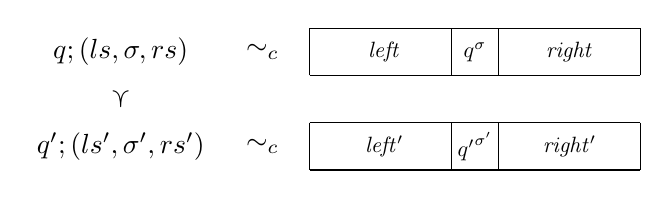
\begin{tikzpicture}[scale=1.2]
    \node at (0, 0.5) {$q; (ls, \sigma, rs)$};
    \node at (0, -0.5) {$q'; (ls', \sigma', rs')$};
    \node[rotate=270] at (0, 0) {$\succ$};

    \draw[scale=0.5] (4, 0.5) -- (11, 0.5);
    \draw[scale=0.5] (4, 1.5) -- (11, 1.5);
    \draw[scale=0.5] (4, 0.5) -- (4, 1.5);
    \draw[scale=0.5] (11, 0.5) -- (11, 1.5);

    \draw[scale=0.5] (7, 0.5) -- (7, 1.5);
    \draw[scale=0.5] (8, 0.5) -- (8, 1.5);

    \node[scale=0.8] at (2.75, 0.5) { $\rev~\mathit{left}$ };
    \node[scale=0.8] at (4.75, 0.5) { $\mathit{right}$ };
    \node[scale=0.8] at (3.75, 0.5) { $q^\sigma$ };

    \node[rotate=270] at (3.75, 0) {$\rightsquigarrow$};

    \draw[scale=0.5] (4, -0.5) -- (11, -0.5);
    \draw[scale=0.5] (4, -1.5) -- (11, -1.5);
    \draw[scale=0.5] (4, -0.5) -- (4, -1.5);
    \draw[scale=0.5] (11, -0.5) -- (11, -1.5);

    \draw[scale=0.5] (7, -0.5) -- (7, -1.5);
    \draw[scale=0.5] (8, -0.5) -- (8, -1.5);

    \node[scale=0.8] at (2.75, -0.5) { $\rev~\mathit{left'}$ };
    \node[scale=0.8] at (4.75, -0.5) { $\mathit{right'}$ };
    \node[scale=0.8] at (3.75, -0.5) { ${q'}^{\sigma'}$ };

    \node at (1.5, 0.5) {$\sim_c$};
    \node at (1.5, -0.5) {$\sim_c$};
  \end{tikzpicture}
\end{center}
where $ls \sim_t^{p} \mathit{left}, rs \sim_t^{p} \mathit{right}$ and $ls' \sim_t^{p'} \mathit{left'}, rs' \sim_t^{p'} \mathit{right'}$. 
From the existence of a $\succ$ or $\rightsquigarrow$ transition, we get the unique existence of the other transition.

We start off with an important lemma that allows us to split up a rewrite $h \strent{} h'$ into three rewrites involving the center state symbol and a rewrite each for the two tape halves.
\begin{proposition}\label{lem:rewrite_split}
  \begin{align*}
    &(A \concat [c, d, e, f, g] \concat B) \strent{R} (A' \concat [c', d', e', f', g'] \concat B') \land \length{A} = \length{A'} \land \length{B} = \length{B'} \\
    \leftrightarrow& \quad
    \begin{aligned}[t]
      &(A \concat [c, d] \strent{R} A' \concat [c', d']) \\
      \land& ([f, g] \concat B) \strent{R} ([f', g'] \concat B') \\
      \land& \irewwin{c}{d}{e}{c'}{d'}{e'} \in R \land \irewwin{d}{e}{f}{d'}{e'}{f'} \in R\land \irewwin{e}{f}{g}{e'}{f'}{g'}\in R
    \end{aligned}
  \end{align*}
\end{proposition}

Conversely, if we start out with a string of the form given in the previous proposition and rewrite to another string, the new string can also be split up accordingly. 
\begin{proposition}\label{prop:rewrite_split_conv}
  \begin{align*}
    &(A \concat [a, b, c, d, e] \concat B) \strent{} s' \\
    \rightarrow &~\exists A'~B'~a'~b'~c'~d'~e', s = A' \concat [a', b', c', d', e'] \concat B' \land \length{A} = \length{A'} \land \length{B} = \length{B'}
  \end{align*}
\end{proposition}

The following two results are the main correctness statements for the Turing machine simulation.
\begin{lemma}[Step Simulation]\label{lem:stepsim}~\\
  If $(q, tp) \reprc{} s$, $(q, tp) \succ (q', tp')$ and $\length{tp} < z$, then $\mexists s', s \strent{\Rsim} s' \land (q', tp') \reprc{} s'$. 
\end{lemma}
\begin{proof}
  The proof follows the following idea which was already outlined previously: 
  \begin{center}
    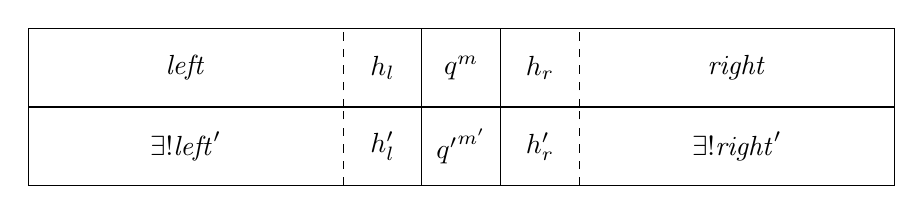
\begin{tikzpicture}
      \draw (0, 0) -- (11, 0);
      \draw (0, 1) -- (11, 1);
      \draw (0, 0) -- (0, 1);
      \draw (11, 0) -- (11, 1);

      \draw (5, 0) -- (5, 1);
      \draw (6, 0) -- (6, 1);

        \draw[dashed] (7, 0) -- (7, 1);
        \draw[dashed] (4, 0) -- (4, 1);
        \node at (4.5, 0.5) {$h_l$};
        \node at (6.5, 0.5) {$h_r$};

      \node at (2, 0.5) {$\mathit{left}$};
      \node at (9, 0.5) {$\mathit{right}$};
      \node at (5.5, 0.5) {$q^m$};

        \draw (4, -1) -- (7, -1);
        \draw (5, -1) -- (5, 0);
        \draw (6, -1) -- (6, 0);

        \draw[dashed] (7, -1) -- (7, 0);
        \draw[dashed] (4, -1) -- (4, 0);

        \node at (4.5, -0.5) {$h_l'$};
        \node at (6.5, -0.5) {$h_r'$};
        \node at (5.5, -0.5) {${q'}^{m'}$};

        \draw (0, -1) -- (0, 0);
        \draw (11, -1) -- (11, 0);
        \draw (0, -1) -- (4, -1);
        \draw (7, -1) -- (11, -1);

        \node at (2, -0.5) {$\exists! \mathit{left}'$};
        \node at (9, -0.5) {$\exists! \mathit{right}'$};
    \end{tikzpicture}
  \end{center}
  Given a configuration string, we split it into the state symbol $q^m$, the left tape half, and the right tape half. The state symbol uniquely determines the transition the Turing machine takes. By analysing the heads $h_l$ and $h_r$ of the tape halves, we can find out the rewrite windows to use at the center. 
  These windows then uniquely determine the heads $h_l'$ and $h_r'$ of the successor tape halves. 
  Using Lemmas~\ref{lem:tape_add}-\ref{lem:tape_stay}, the successor tape halves are therefore fully determined. 
  The rewrites can be justified seperately by Lemma~\ref{lem:rewrite_split}.

  We have to do several case analyses on the transition that is taken and the shape of the left and right tape halves. As an example, we look at the case where $m = \OSome{\sigma}$ and $\delta(q, \OSome{\sigma}) = (q', \OSome{\sigma'}, \movel)$, $\tmleft{tp} = \rev{(\sigma_1 :: \sigma_2 :: left')}$, $\tmright{tp} = \sigma_3 :: right'$. 
  By assumption, there are $h_1 = \sigma_1^{p} :: \sigma_2^{p} :: h_1'$, $h_2 = \sigma_3^p :: h_2'$ with $\sigma_1 :: \sigma_2 :: left' \reprtt{z}{p} h_1$ and $\sigma_3 :: right' \reprtt{z}{p} h_2$. 
  Pictorially, the tape looks as follows:
  \begin{center}
    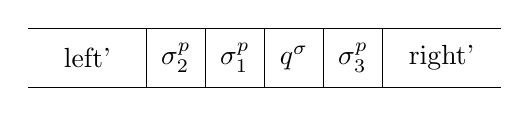
\begin{tikzpicture}
      \draw (0, 0.75) -- (6, 0.75);
      \draw (0, 0) -- (6, 0);
      \draw (1.5, 0) -- (1.5, 0.75);
      \draw (2.25, 0) -- (2.25, 0.75);
      \draw (3, 0) -- (3, 0.75);
      \draw (3.75, 0) -- (3.75, 0.75);
      \draw (4.5, 0) -- (4.5, 0.75);
      
      \node at (0.75, 0.375) {left'};
      \node at (1.875, 0.375) {$\sigma_2^p$};
      \node at (2.625, 0.375) {$\sigma_1^p$};
      \node at (3.375, 0.375) {$q^\sigma$};
      \node at (4.125, 0.375) {$\sigma_3^p$};
      \node at (5.25, 0.375) {right'};
    \end{tikzpicture}
  \end{center}
  Thus, we apply the window 
  \begin{center}
    \trewwin{\sigma_1^p}{q^{\sigma}}{\sigma_3^p}{\polpos{\sigma_2}}{{q'}^{\sigma_1}}{\polpos{\sigma'}}
  \end{center}
  at the center.
  Doing one more case analysis for the left and right tape halves, we can determine the other two rewrite windows to use at the center.

  Next, we transform the two halves of the tape. The element $\sigma_1$ needs to be removed from the left tape half, while $\sigma'$ needs to be added to the right tape half. 
  By Lemma~\ref{lem:tape_rem}, there is a unique $h_1''$ such that 
  \begin{align*}
    \rev{(\sigma_1^p :: \sigma_2^p :: h_1)} \strent{} \rev{(\polneg{\sigma_2} :: h_1'')} \text{ and } \sigma_2 :: left' \reprtt{+}{z} \polpos{\sigma_2} :: h_1''. 
  \end{align*}
  Similarly, by Lemma~\ref{lem:tape_add}, there is a unique $h_2''$ such that
  \begin{align*}
    \sigma_3^p :: h_2' \strent{} \polpos{\sigma'} :: \polpos{\sigma_3} :: h_2'' \text{ and } \sigma' :: \sigma_3 :: right' \reprtt{+}{z} \polpos{\sigma'} :: \polpos{\sigma_3} :: h_2''. 
  \end{align*}

  These two results can be used to justify the rewrite for the two tape halves. Moreover, we have to show that 
  \begin{align*}
    (q', tp') \reprc{} \rev{(\polpos{\sigma_2} :: h_1'')} \concat [{q'}^{\sigma_1}] \concat (\polpos{\sigma'} :: \polpos{\sigma_3} :: h_2''), 
  \end{align*}
  which is straightforward, as $tp' = \textsf{doAct}~tp~(\OSome{\sigma'}, \movel)$, i.e.
  \begin{align*}
    tp' = \textsf{midtape}~(\sigma_2 :: left')~\sigma_1~(\sigma' :: \sigma_3 :: right').
  \end{align*}

  Finally, we prove that the rewrite is unique. Assuming that the current configuration string rewrites to $s'$, we can also split up $s'$ along the state symbol by Proposition~\ref{prop:rewrite_split_conv}. We do an inversion on the rewrite windows used at the center, applying Lemmas~\ref{lem:sim_inv1} and ~\ref{lem:sim_inv2} in the process, and then use the uniqueness for both tape halves.
\end{proof}

\begin{lemma}[Halting Simulation]\label{lem:haltsim}~\\
  If $(q, tp) \reprc{} s$, $\textsf{halt}~q = \btrue$, then $\mexists s', s \strent{\Rsim} s' \land (q, tp) \reprc{} s'$.
\end{lemma}
\begin{proof}
  Using a similar style of arguments as for Lemma~\ref{lem:stepsim}, but simpler, as we do not have to handle all the cases of the transition function.
\end{proof}

\section{Deterministic Simulation}
We extend the results of the previous section to cover multiple simulation steps and define a set of final substrings. In the end, we obtain that, starting from any input, the resulting \PR{} instance does exactly simulate the Turing machine.

\subsection{Multi-step Simulation}
If there is enough space left on the tape, the rewrite windows $\Rsim$ can exactly act like the Turing machine.

\begin{lemma}[Multi-step Completeness]\label{lem:multistep_complete}
  Let $(q, tp) \reprc{} s$, $(q, tp) \succ^i (q', tp')$ for some $z \ge i \ge 0$, and $\length{tp} \le z - i$, then $\mexists s', s \strent{\Rsim}^i s' \land (q', tp') \reprc{} s'$. 
\end{lemma}
\begin{proof}
  By induction on $(q, tp) \succ^i (q', tp')$, using Lemma~\ref{lem:stepsim} in the successor case. 
\end{proof}

\begin{remark}
  At this point, our choice to have a fixed state symbol (head) position finally pays off. If we had chosen to use a moving head semantics, we would now need an additional invariant stating that the state symbol is at least $i$ symbols away from the border of the string. This would need to be built-in into the representation relations, requiring an additional parameter for $\reprt{}, \reprc{}$ determining the amount of available space.
  The requirement $\length{tp} \le z - i$ which only talks about the tape that is represented is much simpler.
\end{remark}

\begin{lemma}[Multi-step Halting]\label{lem:multistep_halt}
  If $(q, tp) \reprc{} s$, $\textsf{halt}~q = \btrue$, then $\mexists s', s \strent{\Rsim}^i s' \land (q, tp) \reprc{} s'$. 
\end{lemma}

\begin{lemma}[Multi-step Soundness]\label{lem:multistep_sound}
  If $(q, tp) \reprc{} s$, $i \le z$, $\length{tp} \le z - i$, and $s~\strent{\Rsim}^i~s'$, then there exist $q', tp'$ and $j$ with 
  \begin{itemize}
    \item $(q', tp') \reprc{} s'$, 
    \item $j \le i$, 
    \item $(q, tp) \succ^j (q', tp')$, 
    \item and $\length{tp'} \le \length{tp} + j$.
  \end{itemize}
\end{lemma}
\begin{proof}
  Logically, a new line is appended to the tableau of configurations with each rewrite step. Thus, a direct induction over $s~\strent{\Rsim}^i s'$ fails: the definition of $\strent{\Rsim}^i$ prepends a new line with each step. By Proposition~\ref{prop:relpower}, we switch to $\prescript{i}{}{\strent{\Rsim}}$. 
  Now, the induction goes through. In the successor case, we make a case analysis on $\textsf{halt}~q$ (which is also the reason why the naive induction fails).
\end{proof}

\subsection{Soundness and Completeness}
We do not directly define the set of final substrings according to the definition of \PR{}, but instead work with a more abstract notion for now.

\begin{definition}[Halting String]
  \[\haltString{s} \defeq \exists p~m, p^m \in s \land \textsf{halt}~p = \btrue \]
\end{definition}

\begin{lemma}\label{lem:finalcond}
  If $(q, tp) \reprc{} s$, then $\textsf{halt}~q = \btrue$ if, and only if, $\haltString{s}$. 
\end{lemma}

We now obtain soundness and completeness of the full simulation.
\begin{theorem}[Completeness]
  If $\length{tp} \le k$, $(q, tp) \reprc{} s$, and $(q, tp) \rhd^{\le  t} (q', tp')$, then there is $s'$ with $s \strent{}^t s'$, $(q', tp') \reprc{} s'$ and $\haltString{s'}$. 
\end{theorem}
\begin{proof}
  By Lemmas~\ref{lem:multistep_complete},~\ref{lem:multistep_halt}, and~\ref{lem:finalcond}.
\end{proof}


\begin{theorem}[Soundness]
  If $(q, tp) \reprc{} s$, $\length{tp} \le k$, $s \strent{}^t s'$, and $\haltString{s'}$, then there are $q', tp'$ with $(q', tp') \reprc{} s'$, $(q, tp) \rhd^{\le t} (q', tp')$ and $\length{tp'} \le z$. 
\end{theorem}
\begin{proof}
  By Lemmas~\ref{lem:multistep_sound} and~\ref{lem:finalcond}.
\end{proof}

Next, we define valid initial strings and concretise the final substrings. 
For the definition of initial strings, we use the notion of valid initial tapes introduced in Definition~\ref{def:tmgennp}.

\newcommand{\initString}{\textsf{initialString}}
\newcommand{\isInitString}{\textsf{isInitialString}}

\begin{definition}[Initial Strings]
  \begin{align*}
    \mnotec{\initString}~c \defeq \stringForConfig~q_0~(\textsf{initTape}~(in \concat c)) \\
    \mnotec{\isInitString}~s \defeq \exists s', s = \initString~s' \land \validCert{s'}
  \end{align*}
\end{definition}

\begin{definition}[Final Substrings]
  \mnote{$\Rfinal$}
  \[\Rfinal \defeq \withl q^m \withm \textsf{halt}~q = \btrue \withr \]
\end{definition}

\begin{proposition}
  \[ s \models \Rfinal \leftrightarrow \haltString{s} \]
\end{proposition}

We have now reduced \gennp{} to the following question: 
\begin{problem}\label{prob:exinput}~\\
  Given a string $s$ with $\isInitString~s$, does $\PR{}~(\Gamma, 1, 3, s, \Rsim, \Rfinal, t)$ hold?
\end{problem}

\section{Interlude: Nondeterministic Preludes}\label{sec:preludes}
In this section, we give a recipe to reduce existential questions as in Problem~\ref{prob:exinput}, where the initial string of a \PR{} instance is unknown, to full \PR{} instances with a fixed initial string. 
While all rewrite windows seen so far only allowed for deterministic rewriting, the key is to make the rewrite windows nondeterministic. The results presented here can also be seen as providing a (very limited) form of compositionality for \PR{}.

The construction works by adding new rewrite windows and a new initial string, which together form a \emph{prelude} to the given \PR{} instance. 
Of course, we have to make sure that the new windows do not interfere with the ``old'' ones. To a large part, this can be ensured syntactically by expanding the alphabet. Additionally, we require the rewrite windows to produce a string of the old alphabet in exactly $t'$ steps, which we call the number of \emph{prelude steps}. 

We present the results for the special case of 3-\PR{}, albeit they transfer directly to the more general setting.

The following definition generalises the question stated by Problem~\ref{prob:exinput}.
\newcommand{\expr}{\textbf{Ex3PR}}
\begin{definition}[Existential 3-\PR{} (\expr{})]
  \mnote{\expr{}}
  Given a 3-\PR{} instance $(\Gamma, l, R, \Rfinal, t)$ missing an input, where $l$ denotes the desired input length, and a predicate $p : \listsof{\Gamma} \rightarrow \Prop$, \expr{} is defined as follows:
  \[\expr{}~(\Gamma, l, R, \Rfinal, t)~p \defeq \exists s, \length{s} = l \land p~l \land \PR{}~(\Gamma, 1, 3, s, R, \Rfinal, t) \]
\end{definition}

Let us fix an \expr{} instance $S = (\Gamma, l, R, \Rfinal, t)$ over input predicate $p$. 
Moreover, let a \emph{prelude alphabet} $\Delta : \finType$, a list of prelude windows $R' : \listsof{(\textsf{window}~\Delta~(\Gamma + \Delta))}$, a number of prelude steps $t'$, and an initial string $x_0 : \listsof{\Delta}$ be given. Collectively, we refer to $(\Delta, R', t', x_0)$ as a \emph{prelude}. 
Here, the new notation $\textsf{window}~\Delta~(\Gamma + \Delta)$ means that the premises of the windows are over type $\Delta$, while the conclusions are over type $\Gamma + \Delta$. The latter is necessary because the prelude should eventually generate an input for $S$, while the new windows should not be applicable to strings of the original instance after the prelude has finished.

The alphabet of the new \PR{} instance will be $\mathcal{A} \defeq \Gamma + \Delta$.\mnote{$\mathcal{A}$}

\newcommand{\isOrigString}{\textsf{origString}}
\newcommand{\isPreludeString}{\textsf{preludeString}}

\mnote{\isOrigString}
Throughout this section, we implicitly lift elements of $\Gamma$ and $\Delta$ to $A$, the same applies to strings and windows over these alphabets. 
Where it is needed, we use the predicates $\isOrigString, \isPreludeString : \listsof{A} \rightarrow \Prop$ to distinguish strings over $\Gamma$ and $\Delta$. 
\mnote{\isPreludeString}

\begin{assumption}[Structural Assumptions on the Prelude]
  We place the following assumptions on $(\Delta, R', t', x_0)$: 
  \begin{description}
    \item[$(A_0)$] $l \ge 3$
    \item[$(A_1)$] $\forall x_0', x_0 \strent{R'}^{t'} x_0' \rightarrow \isOrigString~x_0'$
    \item[$(A_2)$] $\forall k~x, k < t' \rightarrow x_0 \strent{R'}^k x \rightarrow \isPreludeString~x$
    \item[$(A_3)$, Completeness] $\forall x_0', \length{x_0'} = l \land p~x_0' \rightarrow x_0 \strent{R'}^{t'} x_0'$
    \item[$(A_4)$, Soundness] $\forall x_0', x_0 \strent{R'}^{t'} x_0' \rightarrow p~x_0'$ 
    \item[$(A_5)$, Compatibility] $\length{x_0} = l$
  \end{description}
\end{assumption}

Assumption $(A_0)$ is required to avoid vacuous rewriting.
Assumptions $(A_1)$ and $(A_2)$ together express that the initial string $x_0$ rewrites in exactly $t'$ steps to a string to which the original windows $R$ can be applied. Moreover, assumptions $(A_3)$ and $(A_4)$ ensure that the prelude can generate exactly those strings described by the predicate $p$ as an input to $S$.

\newcommand{\Rcomb}{\ensuremath{R_{\text{comb}}}}
Now, we construct a new \PR{} instance $S'$ over alphabet $\mathcal{A}$. We define:
\[S' \defeq (A, 1, 3, x_0, \Rcomb, \Rfinal, t + t')~\text{with}~\Rcomb \defeq R \concat R' \mnote{$\Rcomb$}\]
$S'$ witnesses the reduction of \expr{} to \PR{}: the main goal of this section is to show that 
$\expr{}~p~S \leftrightarrow \PR{}~S'$. From an abstract perspective, the proof is quite simple. 
Most of the formal work is due to the handling of the different alphabets and the injections into the combined alphabet.

We therefore only state the most important intermediate result. Intuitively, this allows us to split a sequence of rewrites in the combined instance $S'$ into $t'$ rewrites due to the prelude and $t$ rewrites due to the original instance $S$. 
\begin{lemma}\label{lem:prelude_split}
  If $x_0 \strent{\Rcomb}^{t' + t} s$, then there exists $x_0'$ with $x_0 \strent{R'}^{t'} x_0'$, $x_0' \strent{R}^t s$ and $\isOrigString~s$. 
\end{lemma}
\begin{proof}
  For the proof, we use the following simple facts:
  \begin{enumerate}[1)]
    \item If $n \le t'$ and $x_0 \strent{\Rcomb}^n b$, then $x_0 \strent{R'} b$. 
    \item If $\length{s} \ge 3$, $\isOrigString~s$, and $s \strent{\Rcomb}^n b$, then $s \strent{R}^n b$ and $\isOrigString~b$. 
  \end{enumerate}
  We apply additivity of $\strent{}^{t+t'}$ (Proposition~\ref{prop:relpower}) to the assumption and choose the the resulting $x_0'$. 
  It is known that $x_0 {\strent{\Rcomb}}^{t'} x_0'$ and $x_0' {\strent{\Rcomb}}^t s$. 
  By 1), $x_0 \strent{R'} x_0'$, which shows the first part of the goal. 
  Applying $(A_1)$, we get $\isOrigString~x_0'$. The proof is closed using 2).
\end{proof}

The main result is now a straightforward consequence.
\begin{theorem}\label{thm:expr_to_pr}
  \[\expr{}~p~S \leftrightarrow \PR{}~S' \]
\end{theorem}
\begin{proof}
  Using Lemma~\ref{lem:prelude_split} and the assumptions.
\end{proof}

\section{Guessing the Certificate}
In this section, we apply the technique presented in Section~\ref{sec:preludes} to ``guess'' an accepted certificate and thus generate a full input for the Turing machine. To that end, we design an initial string and nondeterministic rewrite rules that generate an input in a single rewrite step.

\newcommand{\nblank}{\ensuremath{\underline{\blank}}}
\newcommand{\ndelim}{\ensuremath{\underline{\#}}}
\newcommand{\nstar}{\ensuremath{\underline{*}}}
\newcommand{\ninit}{\ensuremath{\underline{q_0^{\blank}}}}
\newcommand{\nsig}[1]{\ensuremath{\underline{#1}}}

\newcommand{\initStr}{\textsf{initStr}}
\newcommand{\Rprelude}{\ensuremath{R_{\text{prelude}}}}

The alphabet \mnotec{$\Delta$} of the prelude has $4 + \length{\Sigma}$ elements, where $q_0 = \textsf{start}$ is the initial state.
\[\Delta \defeq \nblank \bnfmid \nstar \bnfmid \ninit \bnfmid \ndelim \bnfmid \nsig{\sigma} \qquad \sigma : \Sigma\]
As in the previous section, we implicitly lift $\Delta$ and $\Gamma$ to the combined alphabet $\mathcal{A}\defeq \Gamma + \Delta$. This requires some additional work for the formal proofs which we omit on paper.\mnote{$\mathcal{A}$}

Following Section~\ref{sec:informal_nondet}, the initial string has the following form, where $\underline{in} = \withl \underline{\sigma} \withm \sigma \in in \withr$:
\begin{center}
  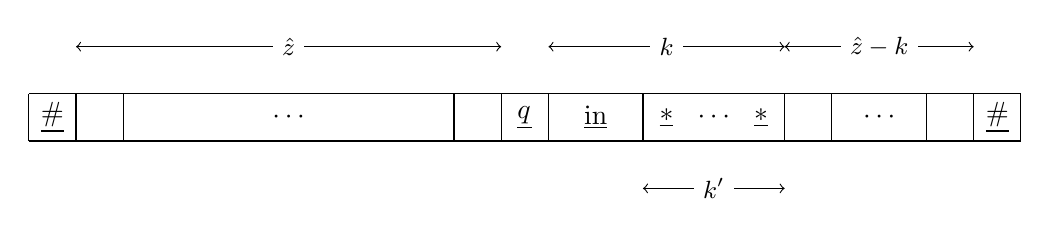
\begin{tikzpicture}[scale=1.2]
    \draw (0, 0.5) -- (10.5, 0.5);
    \draw[thick] (0, 0) -- (10.5, 0);
    \draw (0, 0) -- (0, 0.5);
    \draw (10.5, 0) -- (10.5, 0.5);

    \draw (0.5, 0.5) -- (0.5, 0);
    \draw (1, 0.5) -- (1, 0);
    \draw (10, 0.5) -- (10, 0);
    \draw (9.5, 0.5) -- (9.5, 0);
    \draw (5, 0.5) -- (5, 0);
    \draw (5.5, 0.5) -- (5.5, 0);
    \draw (4.5, 0.5) -- (4.5, 0);
    \draw (6.5, 0.5) -- (6.5, 0);
    %\draw (7, 0.5) -- (7, 0);
    %\draw (7.5, 0.5) -- (7.5, 0);
    \draw (8, 0.5) -- (8, 0);
    \draw (8.5, 0.5) -- (8.5, 0);

    \node at (9, 0.25) {$\cdots$};
    \node at (7.25, 0.25) {$\cdots$};
    \node at (2.75, 0.25) {$\cdots$};

    \node at (0.25, 0.25) {\underline{\#}};
    \node at (0.75, 0.24) {$\underline{\blank}$};
    \node at (4.75, 0.25) {$\underline{\blank}$};
    \node at (5.25, 0.25) {$\underline{q^{\blank}}$};
    \node at (6, 0.25) {\underline{in}};
    \node at (6.75, 0.25) {$\underline{*}$};
    \node at (7.75, 0.25) {$\underline{*}$};
    \node at (8.25, 0.25) {$\underline{\blank}$};
    \node at (9.75, 0.25) {$\underline{\blank}$};
    \node at (10.25, 0.25) {\underline{\#}};

    \path[<->] (5.5, 1) edge node[fill=white, anchor=center, pos= 0.5] {\small $k$} (8, 1);
    \path[<->] (0.5, 1) edge node [fill = white, anchor=center, pos=0.5] {\small $\hat{z}$} (5, 1);
    \path[<->] (8, 1) edge node [fill = white, anchor =center, pos=0.5] {\small $\hat{z}-k$} (10, 1);
    \path[<->] (6.5, -0.5) edge node[fill=white, anchor=center,pos=0.5] {\small $k'$} (8, -0.5);
  \end{tikzpicture}
\end{center}


Let $\initStr : \listsof{\Delta}$ be this initial string.\mnote{$\initStr$}

For the rewrite windows, we have to ensure that all elements of $\Sigma$ are placed contiguously and that inputs of length $< k$ are allowed, too. Exploiting the fact that the rewrite windows overlap, this is easy to achieve.
\begin{center}
  \trewwin{\nblank}{\nblank}{\nblank}{\polneut\blank}{\polneut\blank}{\polneut\blank}
  \quad \trewwin{\ndelim}{\nblank}{\nblank}{\#}{\polneut\blank}{\polneut\blank}
  \quad \trewwin{\nblank}{\nblank}{\ndelim}{\polneut\blank}{\polneut\blank}{\#}\\
  \trewwin{\nblank}{\nblank}{\ninit}{\polneut\blank}{\polneut\blank}{q_0^\blank}
  \quad \trewwin{\nblank}{\ninit}{\nstar}{\polneut\blank}{q_0^\blank}{\polneut{m_1}}
  \quad \trewwin{\nblank}{\ninit}{\nblank}{\polneut\blank}{q_0^\blank}{\polneut\blank}\\
  \trewwin{\ninit}{\nblank}{\nblank}{q_0^\blank}{\polneut\blank}{\polneut\blank}
  \quad \trewwin{\ninit}{\nstar}{\nblank}{q_0^\blank}{\polneut{m_1}}{\polneut\blank}
  \quad \trewwin{\ninit}{\nstar}{\nstar}{q_0^\blank}{\polneut{\sigma_1}}{\polneut{m_1}}
  \quad \trewwin{\ninit}{\nstar}{\nstar}{q_0^\blank}{\polneut\blank}{\polneut\blank}\\
  \trewwin{\nstar}{\nstar}{\nstar}{\polneut{\sigma_1}}{\polneut{\sigma_2}}{\polneut{m_1}}
  \quad\trewwin{\nstar}{\nstar}{\nstar}{\polneut{\sigma_1}}{\polneut\blank}{\polneut\blank}
  \quad\trewwin{\nstar}{\nstar}{\nstar}{\polneut\blank}{\polneut\blank}{\polneut\blank}\\
  \hspace{0.10mm}\trewwin{\nstar}{\nstar}{\nblank}{\polneut{\sigma_1}}{\polneut{m_1}}{\polneut{\blank}}
  \quad\trewwin{\nstar}{\nstar}{\nblank}{\polneut{\blank}}{\polneut{\blank}}{\polneut{\blank}}
  \quad\trewwin{\nstar}{\nblank}{\nblank}{\polneut{m_1}}{\polneut{\blank}}{\polneut{\blank}}
\end{center}
The windows enforce that, if we decide to replace a $\nstar$ with a blank instead of an element of $\Sigma$, all $\nstar$'s to the right of it are also replaced by a blank.
Let \mnotec{$\Rprelude$} denote the set of prelude rewrite windows.

We prove that these rewrite windows exactly produce valid initial strings in a single rewrite step.
In contrast to the Turing machine simulation and the tape rules presented in Section~\ref{sec:taperules}, the prelude does not treat both tape halves symmetrically. 
Therefore, the elegant approach of proving results for the right tape half and afterwards transferring them to the left tape half is not possible. However, for the left tape half we only need to prove that it rewrites exactly to the string representing a blank tape. Everything which is interesting is happening on the right half. 
This is advantageous as we can do simple inductive proofs for the right tape half (in contrast to the left tape half where the reversion is causing trouble). Recall that the right tape half consists of three regions: the fixed input string, the wildcards for the certificate, and a number of blanks. The plan of attack is thus to stack these components on top of each other.


\begin{lemma}\label{lem:prelude_blank}\leavevmode
  We can produce exactly a blank string from a blank prelude string.
  \begin{enumerate}
    \item $\mexists s, \nblank^{\hat{n}} \concat [\ndelim] \strent{\Rprelude} s \land s = \nilstr{(\circ)}{\hat{n}}$
    \item $\mexists s, \rev (\nblank^{\hat{n}} \concat [\ndelim]) \strent{\Rprelude} s \land s = \rev(\nilstr{(\circ)}{\hat{n}})$
  \end{enumerate}
\end{lemma}
\begin{proof}
  For the first statement, existence follows by induction on $n$ and uniqueness follows by a routine induction on $\strent{}$. 
  In order to prove the second statement, we switch to the explicit characterisation (Lemma~\ref{lem:agree_valid}) and do an induction on the index.
\end{proof}

Next, we show that a string starting with a number of wildcards $\nstar$ can be rewritten to either a blank string or a blank string prefixed by a string over $\Sigma$.
\begin{lemma}\leavevmode
  \begin{enumerate}
    \item $\nstar^{n} \concat \nblank^{\hat{j}} \concat [\ndelim] \strent{\Rprelude} \nilstr{(\circ)}{(n + \hat{j})}$
    \item $\nstar^{\length{s}} \concat \nstar^n \concat \nblank^{\hat{j}} \concat [\ndelim] \strent{\Rprelude} \withl \overline{x} \withm x \in s\withr \concat \nilstr{(\circ)}{(n+\hat{j})}$
  \end{enumerate}
\end{lemma}
\begin{proof}
  \begin{enumerate}
    \item Induction on $n$, using Lemma~\ref{lem:prelude_blank} for the base case.
    \item Induction on $s$, using 1.\ for the base case.
  \end{enumerate}
\end{proof}

Of course, we cannot prove uniqueness in this setting. Instead, we prove the following statement.
\begin{lemma}
  \[ \nstar^j \concat \nblank^{\hat{n}} \concat [\ndelim] \strent{\Rprelude} s \rightarrow \exists s', \length{s'} \le j \land s = \withl \overline{x} \withm x \in s \withr \concat \nilstr{(\circ)}{(j + \hat{n})} \]
\end{lemma}
\begin{proof}
  Induction on $j$.
\end{proof}

Lastly, we show that we can prefix the fixed input string to that.
\begin{lemma}\leavevmode
  \begin{enumerate}
    \item $\withl \underline{\sigma} \withm \sigma \in f \withr \concat{} \nstar^{\length{s} + n} \concat{} \nblank^{\hat{j}} \concat{} [\ndelim] \strent{\Rprelude} \withl \overline{x} \withm x \in f \concat{} s\withr \concat{} \nilstr{(\circ)}{(n+\hat{j})}$
    \item $\withl \underline{\sigma} \withm \sigma \in f \withr \concat{} \nstar^j \concat \nblank^{\hat{n}} \concat{} [\ndelim] \strent{} s \rightarrow \exists s', \length{s'} \le j \land s = \withl \overline{x} \withm x \in f \concat{} s \withr \concat{} \nilstr{(\circ)}{(j + \hat{n})} $
  \end{enumerate}
\end{lemma}



This gives us all the tools we need to prove completeness ($A_3$) and soundness ($A_4$) of the prelude.
\begin{lemma}[Completeness]\label{lem:prelude_complete}
  \[ \isInitString~s \land \length{s} = l \rightarrow \initStr \strent{\Rprelude} s \]
\end{lemma}
\begin{proof}
  We do case analysis on the input string $in$ and the number of certificate symbols $k'$ in order to determine five symbols at the center. Then, Lemma~\ref{lem:rewrite_split} allows us to decompose the rewriting. The different cases make use of the previous lemmas.
\end{proof}

\begin{lemma}[Soundness]\label{lem:prelude_sound}
  \[ \initStr \strent{\Rprelude} s \rightarrow \isInitString~s \]
\end{lemma}
\begin{proof}
  Again by doing a case analysis on the symbols at the center and then using the preceding lemmas and inversions. 
\end{proof}

Applying Theorem~\ref{thm:expr_to_pr}, we have now arrived at the full reduction of \gennp{} to 3-\PR{}.

\begin{theorem}[Reduction of \gennp{} to \PR{}]
  \[\gennp~(\Sigma, M, k, t) \leftrightarrow \PR~(\mathcal{A}, 1, 3, \initStr, \Rprelude \concat \Rsim, \Rfinal, 1 + t) \]
\end{theorem}
\begin{proof}
  We have previously reduced \gennp{} to Problem~\ref{prob:exinput}. Theorem~\ref{thm:expr_to_pr} for $t' = 1$ allows us to use the prelude we just constructed to reduce to the \PR{} instance.
  It remains to show assumptions $(A_0) - (A_5)$. 
  The structural requirements $(A_0)$ and $(A_5)$ on the initial prelude string hold by construction. 
  Completeness $(A_3)$ is Lemma~\ref{lem:prelude_complete}, while Soundness $(A_4)$ is Lemma~\ref{lem:prelude_sound}. 
  $(A_2)$ holds trivially as $k < 1$ implies $k = 0$. Finally, $(A_1)$, i.e.\ $\initStr \strent{\Rprelude} x_0' \rightarrow \isOrigString~x_0'$, follows by an easy induction on $\strent{\Rprelude}$ due to the construction of the rewrite windows. 
\end{proof}

\section{Mechanisation}
To close this chapter, we comment on the design choices for the Coq mechanisation and in particular the differences to the presentation on paper. 

\subsection{\PR{}}
First of all, we impose the syntactic constraints (like $\omega > 0$) on \PR{} instances externally, using a predicate $\textsf{PR\_wellformed} : \textsf{PRInstance} \rightarrow \Prop$. 
It is not possible to use a Sigma type, for instance, as this would make the extraction to L impossible. 
Similarly, we do not model windows as elements of type $\Sigma^\omega \times \Sigma^\omega$ using vectors, but instead use lists: $\listsof{\Sigma} \times \listsof{\Sigma}$. The constraint that the lists have length $\omega$ is separate.

In order to ease the mechanisation of the reduction, the variant 3-\PR{} is defined explicitly as a new problem using a separate inductive predicate for validity (cf. Section~\ref{sec:3pr}) and an inductive datatype for storing the three symbols of the premise or conclusion of a window instead of lists.
We then do another reduction from 3-\PR{} to \PR{}, which is just a trivial embedding.

Our definition of validity for 3-\PR{} is parameterised over an abstract $\textsf{rewritesHead} : \listsof{\Sigma} \rightarrow \listsof{\Sigma} \rightarrow \Prop$ predicate which determines whether the prefix of the first list rewrites to the prefix of the second list. The $\textsf{rewHead}$ predicate of Definition~\ref{def:rewHead} is an instance of that.
However, for the proof of the reduction, we use another instantiation: sets of rewrite windows can be alternatively formalised as inductive predicates of type
\[ \Sigma \rightarrow \Sigma \rightarrow \Sigma \rightarrow \Sigma \rightarrow \Sigma \rightarrow \Sigma \rightarrow \Prop, \]
with arguments corresponding to the six elements determining a rewrite window. 
Using inductive predicates instead of lists has the huge advantage of easier automation in Coq: inversions are straightforward and proving that a rewrite is possible can be done by \texttt{eauto} with suitable hints.

\subsection{Organisation of Rewrite Rules}
Another debatable decision is the organisation of rewrite rules. Regarding $\Rtape$, we have opted for two inductive predicates $\textsf{shiftRightRules}$ and $\textsf{identityRules}$, which are then combined into $\textsf{tapeRules}$. The definition of $\textsf{identityRules}$ is abbreviated as presented in Section~\ref{sec:taperules} and thus includes spurious windows, while we explicitly make the distinction between $\sigma : \Sigma$ and blanks for \textsf{shiftRightRules}: the spurious windows for shifting make inversions much harder. 
The rules for shifting the tape to the left are \emph{defined} to be the polarity reversion of the right-shifting rules, which makes Lemma~\ref{lem:symm_rtape} almost trivial.

For the transitions, the rules are much more complicated. We have a hierarchy of inductive predicates that organises them (Figure~\ref{fig:orga_rules}). First, we differentiate according to the syntactic form of the read and written symbols. For instance, the inductive predicate for (Some, None) corresponds to transitions of the form $\delta (q, \OSome{\sigma}) = (q', \ONone, a)$. 
Next is a case analysis on the location of the state symbol, and finally, we distinguish between the three types of movement.
It might seem peculiar that we analyse the state symbol location before the movement as the transition function determines the movement but not the location. The reason is that this makes the inversions in the proofs of Lemmas~\ref{lem:stepsim} and~\ref{lem:haltsim} more efficient. Based on the location of the state symbol, one arrives at a contradiction earlier. Moving to this organisation provided a significant reduction in RAM usage when running the proof. 
\begin{figure}
  \begin{center}
    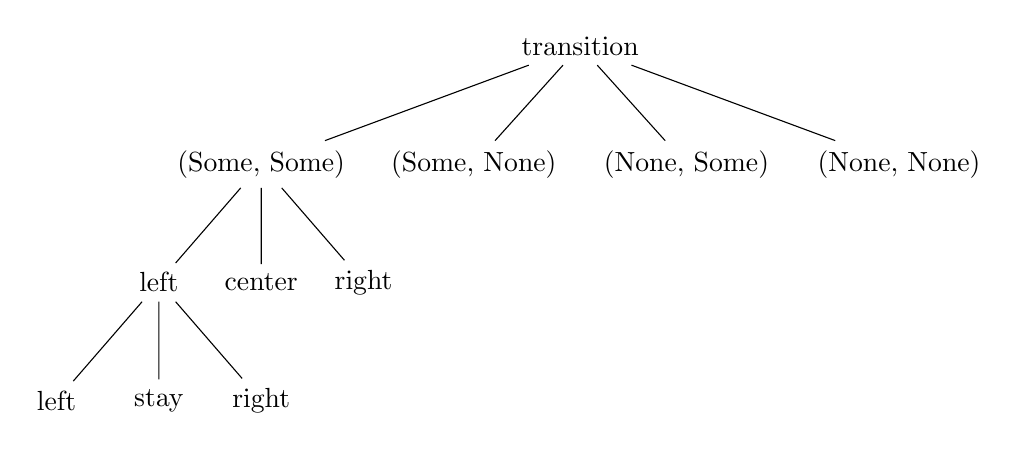
\begin{tikzpicture}[level 1/.style={sibling distance=2.7cm}, level 2/.style={sibling distance =1.3cm}]
      \node {transition}
        child { node {(Some, Some)}
          child {node {left}
            child { node {left} }
            child { node {stay} }
            child { node {right} }
          }
          child {node {center}}
          child {node {right}}
        }
        child {node {(Some, None)}}
        child {node {(None, Some)}}
        child {node {(None, None)}};
    \end{tikzpicture}
  \end{center}
  \caption{The hierarchy of inductive predicates for transitions.}\label{fig:orga_rules}
\end{figure}

The bottom level of the hierarchy can be shared among all four cases except for (None, None), where we need the special handling for the edge of the used tape region. Moreover, for all cases but the (None, None) case, we implement the simplified rules. The spurious windows do not result in any complication in the proofs.

As noted in the proof outline of Lemma~\ref{lem:stepsim}, the number of cases for this lemma is huge: in the end, there are 100 non-contradictory cases left after analysing the possible transitions the Turing machine can take and accounting for the possible symbols at the heads of the two tape halves. The proof thus heavily relies on automation. There is \texttt{LTac} code that analyses the transition the Turing machine can take, destructs the two tape halves far enough, and then puts together the needed lemmas. Custom tactics to invert the tape representation relation $\reprt{}$ are quite important.
Running the proof takes about 35 minutes\footnote{Measured on an Intel Ivy Bridge Core i7-3740QM @ 3.5GHz with 24GB RAM.} and 4 gigabytes of RAM, despite handwritten inversion lemmas for the second and third level of Figure~\ref{fig:orga_rules}. 

\subsection{List-based Rules}
Of course, one still needs to derive a list-based version of the rewrite rules (i.e.\ a variant from which we can directly compute the list of rewrite windows) in order to do the extraction to L and the accompanying running time analysis. Moreover, the extraction mechanism currently is not able to automatically handle finite types. For the flat extractable version, we thus represent finite alphabets using bounded subsets of $\nat$. 

\begin{definition}[Representation of Finite Types]
  Let $T : \finType$, $t : T$, and $k, n : \nat$. 
  \begin{gather*}
    n \approx T \defeq n = \length{T} \mnote{$n \approx T$}\\
    k \approx_{T, n} t \defeq k = \textsf{index}~t \land n \approx T \mnote{$k \approx_{T, n} t$}
  \end{gather*}
\end{definition}

Using this definition, it is easy to encode type constructors like $\opt{\cdot}$, $\cdot \times \cdot$, and $\cdot + \cdot$, as well as value constructors like $\OSome{\cdot}$, $( \cdot, \cdot)$, and $\textsf{inl}~\cdot$. 

\begin{example}[Encoding of option types]
  We define $\textsf{flatOpt}~t \defeq \natS{t}$, $\textsf{flatSome}~k \defeq \natS{k}$ and $\textsf{flatNone} \defeq 0$. 
  Assuming that $n \approx T$ and $k \approx_{T, n} t$, we have:
  \begin{align*}
  \textsf{flatOpt}~n \approx \opt{T} \quad \textsf{flatNone} \approx_{\opt{T}, \textsf{flatOpt}~n} \ONone \quad \textsf{flatSome}~k \approx_{\opt{T}, \textsf{flatOpt}~n}~\OSome{t} \end{align*}
\end{example}

The proof of agreement of the inductive rules with the flat list-based rules proceeds in two steps: first, we define list-based rules still using finite types and show their agreement with the inductive rules. As the hierarchy of Figure~\ref{fig:orga_rules} does not admit an easy computation of the windows (it is not at all natural to do a case analysis on the position of the state symbol when \emph{computing} the windows), we additionally define the inductive predicates using an alternative hierarchy that closely matches the way the windows can be computed (but is notably slower to invert). The advantage of this approach is that the agreement between the two hierarchies can be proved fully automatically at the level of inductive predicates.
In the second step, the flat list-based rules are defined and it is shown that they agree with the finite-type list-based rules, modulo the representation defined by $\approx$. 

We desire that the finite-type and flat rules are defined in one go, with a minimal effort required to show their agreement.
Moreover, in the end, we also need to instantiate the rules with all concrete elements of $\Sigma$ and with the possible polarities to obtain the list of rewrite windows. 

In order to fulfill these two requirements, we define an abstract version \textsf{fAlphabet} of the alphabet $\mathcal{A}$ that contains ``holes'' where an element of $\Sigma$ or $\Sigma_{\text{state}}$, a state of $Q$, or a polarity has to be placed. 
More specifically, these holes are formalised as variables which can be of type $\Sigma, \Sigma_{\text{state}}, Q, \polarity$. 
Given an environment which provides values for the variables, we have two reification procedures \textsf{reifyFin} and \textsf{reifyFlat} taking an element of \textsf{fAlphabet} either to a representation using the finite type $\mathcal{A}$ or a flat representation using $\nat$.
It is shown that, for environments related by $\approx$, the corresponding outputs of \textsf{reifyFin} and \textsf{reifyFlat} are again related by $\approx$.

We then lift the reification procedures to windows and lists of windows.
For the instantiation of the rules, we generate all possible environments for the given number of variables a rule uses and then instantiate the rule with each of those environments to obtain a rewrite window.
In order to generate the windows for the transitions, this needs to be combined with an iteration over all states and elements of $\Sigma_{\text{state}}$, doing a case analysis on the transition function for every valuation.

The proof of agreement with the inductive rules can mostly be automated and only requires the manual choice of an assignment to the variables of a rule.

Finally, we have a separate variant of 3-\PR{} that uses the flat encoding of finite types. The agreement of this flat variant with 3-\PR{} using finite types proceeds in a similar way as in Chapter~\ref{chap:ksat_clique}.\todo{more on that?}
The reduction produces an instance of this flat variant, where the flat reification of the rewrite windows is used. 

\todo{maybe diagram of the logical reduction}

%\todo{comment on design choice of blanks having polarities: makes inversions and generation of list-based rules a whole lot easier}
